\documentclass{xmgr}

\usepackage{minted}
\usepackage{xcolor}
\usepackage{listings}
\usepackage{caption}
\DeclareCaptionFormat{myformat}{#1#2#3}
\captionsetup{format=myformat}
\captionsetup[lstlisting]{position=bottom,format=myformat}
\lstset{basicstyle=\ttfamily,
  showstringspaces=false,
  commentstyle=\color{red},
  keywordstyle=\color{blue}
}

%\defaultfontfeatures{Scale=MatchLowercase}
%\setmainfont[Numbers=OldStyle,Ligatures=TeX]{Minion Pro}
%\setsansfont[Numbers=OldStyle,Ligatures=TeX]{Myriad Pro}
% for fontspec version < 2.0
\setmainfont[Numbers=OldStyle,Mapping=tex-text]{Minion Pro}
\setsansfont[Numbers=OldStyle,Mapping=tex-text]{Myriad Pro}
%\setmonofont[Scale=0.75]{Monaco}

% Opcjonalnie identyfikator dokumentu
% drukowany tylko z~włączoną opcją 'brudnopis':
\wersja   {wersja wstępna [\ymdtoday]}

\author   {Mateusz Kwiatkowski}
\nralbumu {194\,925}
\email    {emflover@gmail.com}

\kierunek{\textbf{INFORMATYKA}}

\title    {Walidacja w~elektronicznym systemie zarządzania osiągnięciami studenta}
\date     {2015}
\miejsce  {Gdańsk}

\opiekun  {dr Włodzimierz Bzyl}

% dodatkowe polecenia

\begin{document}

\begin{abstract}



\indent \indent Pracę poświęcono zagadnieniu walidacji, kwestii ważnej i~integralnie związanej z~odpowiednim funkcjonowaniem sieci.
W szczególności zwrócono uwagę na aspekt prawidłowego zarządzania jej jakością, co obligatoryjnie wiąże się z~problemem
odpowiedniego zabezpieczenia i~odpowiedzialnego korzystania z~niej.
\\
\indent Praca prezentuje sposób tworzenia oraz funkcjonowanie pakietu walidującego do frameworka \textit{Meteor}. Pakiet ten
ma uniemożliwić użytkownikowi wprowadzenie błędnych danych do systemu, dzięki czemu podniesiony zostanie poziom zaufania
do korzystania z~niego. Jednocześnie, aby przybliżyć i~zademonstrować jego działanie, utworzono na potrzeby pracy, aplikację elektroniczny indeks.
Wybór dokumentu nie był przypadkowy. Świadczy o~tym jego wysoka ranga wśród uczelnianej dokumentacji urzędowej. Inny, równie istotny powód
wyboru stanowi fakt, iż korzystanie z~sieci komputerowej w~systemie edukacyjnym stało sie powszechne. Uczelnie wyższe wykorzystują sieć, by
między innymi ułatwić kontakty na linii: wykładowca - student - administracja uczelni.  Temu ma służyć wprowadzenie w~ostatnich latach przez
większość uczelni wyższych w~Polsce, w~tym Uniwersytet Gdański, elektronicznego systemu zarządzania osiągnieciami studentów
tzw. elektronicznego indeksu.
\\
\indent W pracy, walidacji zostaną poddane operacje, które można wykonać w~aplikacji elektroniczny indeks. Do stworzenia jej użyto frameworku \textit{Meteor}, a~dane wprowadzone do systemu, w~celu ich przechowywania umieszczono w~bazie danych - \textit{MongoDB}.

\indent Założono, że skutkiem tego działania będzie uproszczenie, a~nawet intuicyjność obsługi oprogramowania. Cele założone przez autora pracy zostały zrealizowane, czego dowodem jest udostepnienie do pobrania pakietu walidacji systemu.

\end{abstract}
%\keywords{SGML,
% dokumenty strukturalne}

% tytuł i~spis treści
\maketitle
%
% wstęp
\introduction

\indent \indent Najcenniejszym walorem komputera i~Internetu są przechowywane w~nich dane - zarówno
ich ilość, jak i~jakość. Ze względu na to, z~dnia na dzień, rośnie liczba
użytkowników sieci. Jednocześnie zwiększa się liczebność i~różnorodność usług
sieciowych.
\\
\indent Komputer i~Internet zmienił, wciąż zmienia naszą codzienność. To prawda oczywista.
Usługi internetowe nie są już domeną urzędów, firm czy handlu. Chcemy za ich pomocą
robić zakupy, obsługiwać konto w~banku, a~także załatwiać wszelkie formalności w
urzędach. Jest to po prostu wymóg rozwoju cywilizacji, techniki oraz oszczędności
czasu.
\\
\indent Coraz częściej systemy informatyczne wykorzystywane są w~edukacji społeczeństwa.
Jeszcze do niedawna na wszystkich uczelniach wyższych stosowano klasyczne indeksy
papierowe, aby zarchiwizować osiągnięcia studentów podczas całego cyklu kształcenia.
Jednak w~wyniku rozwoju technologii internetowych coraz częściej rezygnuje się
z klasycznych rozwiązań, zastępując je ich elektronicznymi odpowiednikami.
\\
\indent Dziś wiele szkół i~uczelni wprowadziło do obszaru swego funkcjonowania nowoczesny
system ewidencji osiągnięć ucznia czy studenta. W~szkołach podstwowych, gimnazjach,
liceach, technikach czy zasadniczych szkołach zawodowych jest nim tzw. dziennik
elektroniczny. W~uczelniach wyższych  nazwano go elektronicznym indeksem. Zjawisko
to stanowi nie lada wyzwanie, ponieważ wiąże się z~problemem niezawodnego świadczenia
usług w~sieci komputerowej. Odbiorca, w~tym przypadku uczeń lub student, musi mieć
pewność, że dane są stałe, prawdziwe, odpowiednio zabezpieczone przed ich utratą
czy nieuprawnionym dostępem. Należy nadmienić, że taki poziom zaufania i~poczucia
bezpieczeństwa funkcjonowania systemu, powinna mieć również druga strona - nadawca,
ten który wprowadza owe dane. Jest to tym bardziej ważną kwestią, gdyż coraz częściej
mamy do czynienia ze zdarzeniami, wskazującymi na nieprawidłowe stosowanie sieci
komputerowej lub jej nadużycie.
\\
\indent Rozwiązaniem, które zapewniłoby wzrost poziomu zaufania do korzystania
\\
z sieci,
w tym również z~elektronicznego systemu zarządzania osiagnieciami ucznia lub studenta
jest, według autora niniejszej pracy, odpowiednie i~odpowiedzialne zarządzanie jej
jakością, czemu służy walidacja systemu.
\\
\indent Zjawisko to jest szeroko stosowane w~technice i~informatyce. Internetowy Słownik
Języka Polskiego wyjaśnia hasło ,,walidacja'' w~następujacy sposób: ,,walidacja
(technika) - badanie odpowiedności, trafnośc lub dokładności czegoś''.\cite{ValidationSJP}
\\
\indent Sam termin - ,,walidacja'' pochodzi od angielskiego słowa ,,validate'' i~oznacza -
w kontekście informatycznym - sprawdzanie poprawności i~zgodności z~zadanymi
kryteriami. Jest on stosowany w~odniesieniu do danych pochodzących od użytkownika,
jak również w~stosunku do zmiennych, obiektów, typów i~klas w~różnych językach
programowania.\cite{ValidationTermin}
\\
\indent Walidacja jest działaniem, mającym na celu potwierdzenie w~sposób udokumentowany
i zgodny z~założeniami, że procedury, procesy, urządzenia, materiały, czynności
i systemy, rzeczywiście prowadzą do zaplanowanych wyników. Znana jest także jako
kontrola jakości oprogramowania.\cite{Validation2}
\\
\indent Wprowadzając dane do systemu, użytkownik może - świadomie lub nie - popełnić
pomyłkę. Jeżeli dane odebrane przez użytkownika poddamy przetworzeniu bez weryfikacji,
wówczas, w~zależności od odporności aplikacji, możemy mieć do czynienia z~różnymi
rodzajami błędów, od drukowania w~przeglądarce klienta komunikatów diagnostycznych,
poprzez utratę spójności bazy danych, aż po ujawnienie niepowołanym użytkownikom
informacji poufnych. Z~tego powodu nie wolno ignorować wagi problemu.
\\
\indent Aplikacje pozbawione walidacji pozwalają użytkownikowi na wprowadzenie irracjonalnych
danych do systemu. Przykładem takiej aplikacji jest wspomiany przez autora pracy,
elektroniczny indeks. Operacje, takie jak: wystawianie studentowi ocen z~ćwiczeń
czy też oceny z~egzaminu kończącej edukację z~danego przedmiotu, powinny być
odpowiednio walidowane. Dzięki temu nie dojdzie do niepożądanych zjawisk typu:
\begin{itemize}
\item student nie uzyskał pozytywnej oceny z~ćwiczeń, a~otrzymuje ocenę z~egzaminu
kończącego przedmiot,
\item student otrzymuje ocenę spoza skali oceniania systemu danej uczelni,
\item student uzyskuje ocenę od osoby nieuprawnionej do jej wystawienia.
\end{itemize}

Dlatego też, autor pracy chce zwrócić uwagę na rodzący się problem, związany
z wprowadzeniem przez uczelnie elektronicznego indeksu oraz jego odpowiednim
funkcjonowaniem. Zaproponowanie zastosowania walidacji w~elektronicznym systemie
wystawiania ocen usprawni działanie oraz udoskonali jego funkcjonalność.
Korzystając z~aplikacji, w~której zaimplementowana jest walidacja możemy mieć pewność,
że nie dojdzie do sytuacji, by użytkownik wprowadził błędne dane do systemu.
Należy również zwrócić uwagę na ekonomiczny aspekt walidacji. Mianowicie oszczędność
czasu użytkownika czy zwiększenie efektywności jego pracy.
\\
\indent W celu ukazania i~udowodnienia przydatności walidacji podczas korzystania
z elektronicznego systemu zarządzania osiągnięciami studenta, pokazano w~pracy
działanie tego zjawiska w~aplikacji stworzonej w~frameworku \textit{Meteor} oraz
zaprezentowano ułożony pakiet oraz wyjaśniono, jak udostępnić go w~prosty, jasny i~zrozumiały sposób.
\\
\indent Tworzenie pakietu walidującego oraz aplikacji - elektroniczny indeks, która korzysta
ze stworzonego w~ramach pracy pakietu, oparto na doświadczeniu innych badaczy,
zajmujących się oprogramowaniami komputerowymi, takich jak: Kelly Copley, Tom
Coleman czy Sacha Greif. W pracy umieszczono ponadto uzasadnienie, dlaczego wybrane
technologie, takie jak - \textit{Meteor} oraz \textit{MongoDB}, to najbardziej trafny wybór do generowania
pakietu walidacyjnego elektronicznego zarządzania osiągnięciami studenta.
\\
\indent Autor niniejszej pracy miał kontakt z~wieloma systemami zarządzania osiągnieciami
studentów, ale w~każdym można było doprowadzać do anomalii. Zajęcie się rozwiązaniem
tego problemu jest, z~punktu widzenia informatyka interesujące. Efektem pracy może być
nie tylko usprawnienie działania systemu, ale również poczucie, że praca z~nim jest
prosta, przyjemna i~wręcz intuicyjna.

\chapter{Walidacja oprogramowania}

\indent \indent \indent W testowaniu oprogramowania ważne są pojęcia – weryfikacja i~walidacja. Pojęcie walidacji wyjaśniono we wprowadzeniu oraz rudymencie podrozdziału pierwszego. Należy wyjaśnić również pojęcie \textit{weryfikacji}

\textit{Internetowy Słownik Języka Polskiego} podaje następujące znaczenia tego słowa: \textit{weryfikacja} z~łac. \textit{verifico} - ,,wycenić wartość, ustalić; 1. Sprawdzenie zgodności czegoś z~prawdą; sprawdzenie autentyczności czegoś; weryfikacja hipotezy, teorii, faktów. 2. Sprawdzanie i~ocena czyichś kwalifikacji - np. pracownika''. Różnica w~znaczeniu tych pojęć jest istotna. Aby ją wskazać należy zwrócić uwagę na celowość tych dwóch określeń. Specyfika działania weryfikacji to zastosowanie pytania: \textit{,,Czy produkt tworzony jest prawidłowo?''}. Z kolei dla procesu walidacji typowym pytaniem będzie: \textit{,,Czy tworzony produkt jest prawidłowy?''}. \textit{Prawidłowy} – to znaczy zgodny z~wytycznymi programowania, przy zastosowaniu odpowiednich metod, języka programowania i~algorytmów. 

Pojęcia weryfikacji i~walidacji są znaczeniowo na tyle bliskie, że mogą przysporzyć trudności. Zarówno weryfikacja jak i~walidacja produktu są czynnościami, które służą sprawdzeniu, czy wytworzony produkt jest taki, jaki sobie życzyliśmy my, bądź inny interesariusz. \textit{Produkt} możemy rozumieć jako: 

\begin{itemize}
  \item[-] dany moduł systemu,
  \item[-] blok kodu,
  \item[-] cały system,
  \item[-] istotny dokument, na bazie którego moduł lub system będzie zbudowany.
\end{itemize}

Warto zapamiętać, że obie te czynności zachodzą w~wielu różnych momentach i~mogą pojawić się w~wielu fazach procesu tworzenia systemu. Błędnym będzie zatem rozumienie, np. walidacji, jako jakiegoś etapu wieńczącego budowę systemu.

\begin{figure}[th!]
\centering
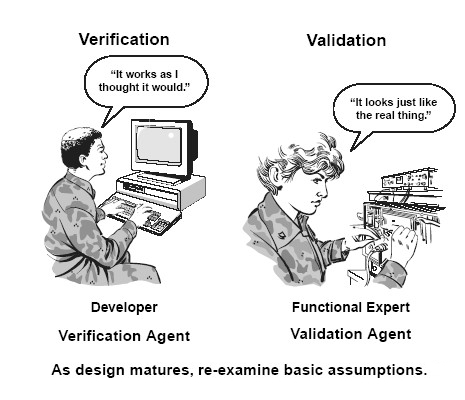
\includegraphics[width=.7\hsize]{images/Verification_Validation_Accreditation}
\caption{Różnice między weryfikacją, walidacją\label{RYS.1}}
\source{http://commons.wikimedia.org/wiki/}
\end{figure}

 Różnice między weryfikacją i~walidacją dotyczą przede wszystkim tego, z~jakiej perspektywy dokonujemy sprawdzenia czy jest to perspektywa technologiczna i~typowa dla zespołów budujących system, czy raczej z~perspektywy użytkownika końcowego, który nie ma obowiązku rozumieć technicznej strony systemu, z~którego będzie korzystał.
\\
\indent Najprościej jest zapamiętać, że weryfikujemy to, co da się wyliczyć, wykazać logicznie i~nie ma jak zanegować tego, co już zweryfikowane. Przy dobrze spisanych wymaganiach weryfikacji dokonać może każdy człowiek rozumiejący tekst specyfikacji i~wiedzący, jak wykonać test. 
Natomiast walidacja zawsze jest po stronie odbiorcy i to zaspokojenie jego potrzeb jest ostatecznym kryterium sukcesu. Odcinając się od możliwości konsultowania z~klientem spraw dotyczących choćby wygody użytkowania produktu, wytwórcy ryzykują niepowodzenie walidacji.
\\
\indent Weryfikacja produktu procesu polega na dostarczeniu dowodów, że dany produkt spełnia z~d~e~f~i~n~i~o~w~a~n~e wymagania. Można spotkać się też z~objaśnieniami tego terminu mówiącymi, że jest to sprawdzanie „czy aplikacja jest prawidłowo zbudowana”, czy produkty danego etapu produkcji spełniają wymogi założone na początku całego procesu.
Kluczowym słowem jest wyraz -  \textit{zdefiniowane}. Weryfikacja domaga się odniesienia do przesłanek, które spisano w~taki sposób, by można je było sprawdzić w~sposób jednoznaczny. Weryfikacja polega na stwierdzeniu, że dany punkt np. specyfikacji technicznej jest informacją, która w~sposób prawdziwy opisuje dany produkt poddany testowi. W praktyce powinniśmy zatem unifikować weryfikację z~procesem, który zakończy się „zero-jedynkowym” rozstrzygnięciem, decydującym o~tym, że dany produkt wygląda, bądź zachowuje się, bądź jest taki, jak ustalono dla niego w~specyfikacji wszystkich przesłanek. Jeśli na przykład jakąś funkcjonalność można:
\begin{itemize}
  \item[-] sprawdzić poprzez odczytanie wyniku liczbowego, którego ona dostarcza; 
  \item[-] zbadać czy odpowiedź systemu nastąpi w~konkretnie ustalonym czasie;
  \item[-] sprawdzić czy następuje przesłanie odpowiedniego pliku między serwerem a~klientem,
wtedy możemy oczekiwać, że proces sprawdzania tego produktu jest weryfikacją.
\end{itemize}


\begin{figure}[th!]
\centering
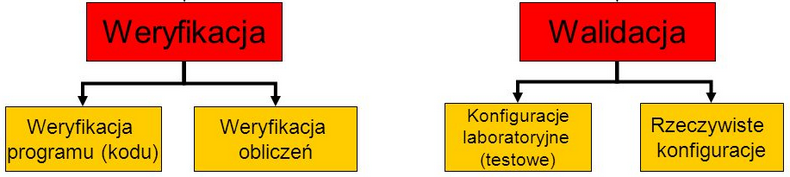
\includegraphics[width=.7\hsize]{images/weryfikacja_walidacja}
\caption{Weryfikacja i~walidacja\label{RYS.2}}
\source{http://slideplayer.pl/slide/427709/ slajd 4}
\end{figure}

\indent Walidacja produktu polega na sprawdzeniu poprawności i~dostarczeniu dowodów,  że proces wytwarzania go, spełnia potrzeby i~wymagania użytkownika. Tłumaczy się ją również, jako „sprawdzenie czy aplikacja jest poprawna” / w~starszych wersjach słowników testerskich / \cite{ALTKOM}
\\
\indent Najistotniejsze do zrozumienia walidacji jest to, że to, co było jasno zdefiniowanym kryterium zaliczenia testu, jest tutaj zamienione na potrzeby i~wymagania użytkownika. O ile zweryfikować można różne rzeczy bez wczuwania się w~rolę użytkownika końcowego / bo wystarczy się oprzeć choćby na wyliczeniach i~sprawdzaniu, czy wyniki są zgodne z~założeniami ze specyfikacji /, to walidacja służy właśnie do sprawdzenia wszystkich tych funkcjonalności, które użytkownik będzie oceniał pod kątem swoich osobistych upodobań, często subiektywnie, nieraz w~oparciu o~rozmaite nawyki.
Sukces walidacji opiera się niejednokrotnie na sprawach, które ciężko jest przewidzieć podczas pisania specyfikacji funkcjonalnej. Odbiorca systemu nieraz nie uświadamia sobie swoich własnych aberracji i~może stwierdzić ich brak dopiero wtedy, gdy przystępuje do finałowego testu akceptacyjnego. Często wtedy słyszanym argumentem z~ust niezadowolonego odbiorcy jest to, że coś było „tak oczywiste, że nie trzeba tego było spisywać w~specyfikacji”.
O ile kluczem do udanej weryfikacji produktu jest klarowne zdefiniowanie kryteriów zaliczenia testu, o tyle kluczem do udanej walidacji jest pogłębiona i~sprawna komunikacja z~odbiorcą, zadawanie celnych pytań pomagających w~zrozumieniu autentycznych potrzeb klienta, przeprowadzanie wraz z~klientem symulacji zastosowań systemu na wszelkiego rodzaju makietach. Kolejną bardzo istotną sprawą jest umiejętne korzystanie z~badań aktualnych rozwiązań i~tendencji w~produktach dostępnych na rynku, co wiąże się z~przeglądaniem odpowiednich stron internetowych, sięganiem po prace znawców tematu i~autorytetów, ciągłym dokształcaniem.
\\
\indent Walidację warto zapamiętać jako ogół tych czynności, które zwiększają szansę na zadowolenie odbiorcy tworzonego produktu i~które będą brały pod uwagę konsultacje z~tym odbiorcą, wspólne wypracowywanie rozwiązania i~przewidywanie jego preferencji.\cite{ALTKOM}

\section{Specjalistyczny wstęp do walidacji}

\indent \indent \indent Walidacja jest to proces wyznaczania kompatybilności stopnia użytkowania systemu, w którym dany model staje się wiernym odzwierciedleniem rzeczywistego systemu. Chodzi o~skuteczną zgodność wprowadzonych danych z~ich oryginałem. Proces ten ma na celu zilustrowanie czy symulacja dostarcza użytkownikowi wiarygodnych danych wyjściowych, zgodnych z~danymi wejściowymi użytkownika. Dokonuje więc, weryfikacji zgodności wizji projektanta z~realnym światem. Pełni rolę autocenzury konkretnego systemu, by każdy wirtualny użytkownik, miał pewność, że dane wprowadzone do systemu są stałe i~spełniają przydzieloną im rolę.
\\
\indent Każdy system informatyczny wymaga osiągnięcia odpowiedniego stopnia adekwatności, bezbłędności, stabilności oraz wyeliminowania błędów działania w~modelu. Przez model, który przeszedł walidację, rozumieć należy ten, który został poddany serii operacji, mających na celu doprecyzowanie go do optymalnego poziomu, przez co, zgodnie z~jego przeznaczeniem, będzie mógł sprostać postawionym przed nim zadaniom. Taki poziom wiarygodności modelu uzyskamy dzięki procesowi walidacji.

Systemy zautomatyzowane i~skomputeryzowane stosowane szczególnie w~przemyśle wysokich technologii, muszą być poddawane okresowym kontrolom, potwierdzającym ich jakość w~celu wykrycia ewentualnych, potencjalnych zagrożeń, wynikających z~bezpośredniego lub pośredniego wpływu na produkt końcowy. Walidacja zatem ma udokumentować, w~jaki sposób należy zmienić i~udoskonalić proces, aby zminimalizować ewentualne skutki jego nieprawidłowego działania.

Jeżeli istnieje możliwość, walidacja systemu powinna być poprzedzona rozmową z~jego użytkownikiem. Ma ona spełnić rolę sondy i~zebrania cennych informacji, by program walidacyjny stał się optymalny. Mając przez długi czas styczność z~systemem rzeczywistym, ekspert często potrafi odpowiedzieć na pytania dotyczące całości systemu lub wskazać rażące błędy, których podstawą jest niezrozumienie rzeczywistego systemu, co staje się przyczyną generowania przez symulację złych wyników. \cite{Validation}

\indent Innym zagadnieniem mającym związek z~procesem walidacji jest problem czasu tworzenia go oraz związanych z~tym kosztów. Walidacja procesów,systemów czy urządzeń jest czasochłonna. Tworzenie dokumentacji, procedur, wykonywanie testów i~działań naprawczych na ogół przeciąga się w~czasie. Dobrze zarządzana walidacja, obciąża budżet projektu w~skali 4 - 7 \% kosztów. Nieprawidłowo prowadzona podnosi ją do 20 – 30\% kosztów całkowitych. Poniesienie niskich nakładów może przynieść wymierne zyski ekonomiczne już w~krótkiej perspektywie. Według danych zgromadzonych przez osoby zajmujące się walidacją dla nowych urządzeń i~systemów produkcyjnych, wydajność początkowa urządzenia, które były przedmiotem pełnego cyklu walidacji, może być 2 – 3 razy wyższa, niż tych uruchomionych bez jej przeprowadzania. Mechanizmy i~systemy poddane walidacji osiągają pełną zdolność produkcyjną a~ich kultura obsługi i~serwisu jest wysoka, ponieważ w~czasie testów walidacyjnych pracownicy zdobywają praktyczną wiedzę od dostawcy czy użytkownika. Właściwe opracowanie \textit{specyfikacji wymagań użytkownika}
\\
/ w~skrócie URS / \footnote{ang. User Requirements Specification - URS}, prowadzenie kwalifikacji projektu, nadzorowanie i~współpraca z~dostawcą od początku wiąże się z~nakładami. Jednak poniesione koszty są niewspółmierne niższe od kosztów poprawy pracy czy usuwania usterek w~gotowym urządzeniu, czy utworzonym systemie. Dlatego ważna jest współpraca z~dostawcą / użytkownikiem  od samego początku inwestycji. Wspólne rozwiązywanie problemów, tworzenie scenariuszy testowych, pozwala na obustronną wymianę wiedzy
\\
i znaczne ograniczenie kosztów w~późniejszej eksploatacji systemu i~urządzenia.\cite{ekonomia}

\section{Kategorie walidacji}

Kryterium funkcjonalności wyróżnia następujący podział walidacji:

\begin{enumerate}
  \item \textbf{\textit{Walidacja prospektywna}} – zadaniem takiej walidacji jest, aby przed wprowadzeniem nowych produktów na rynek upewnić się, że funkcjonują prawidłowo i~spełniają standardy bezpieczeństwa.
  \item \textbf{\textit{Walidacja retrospektywna}} – ten proces wyasygnowano dla produktów, które są już w~użyciu oraz dystrybucji czy produkcji. Walidację tą przeprowadza się na podstawie wcześniej określonych oczekiwań specyfikacji produktu oraz danych historycznych. Jeśli jakiekolwiek dane krytyczne są niepełne, to nie mogą być one przetworzone lub mogą być przetworzone częściowo. Zadania są uważane za konieczne, gdy:
\begin{itemize}
\item walidacja prospektywna jest niewystarczająca lub błędna,
\item zmiana przepisów prawnych lub norm wpływa na zgodnośc produktów wypuszczonych na rynek,
\item przywrócenie produktu do użytkowania.
\end{itemize}
  \item \textbf{\textit{Rewalidacja}} – przeprowadza się dla produktu, który został odrzucony, naprawiony, zintegrowany, przeniesiony lub po upływie określonego czasu.\cite{Categories}
\end{enumerate}

\section{Etapy walidacji}
\indent \indent \indent Zakres walidacji powinien uwzględniać wiele czynników systemu, w tym jego zamierzone zastosowanie i~rodzaj walidacji oraz czy mają być dołączane nowe elementy systemu. Walidacja powinna być uznawana za część całego cyklu użytkowania systemu komputerowego. Obejmuje on planowanie, specyfikację, programowanie, badanie, odbiór techniczny, dokumentację, działanie, monitorowanie i~modyfikowanie.

\begin{figure}[th!]
\centering
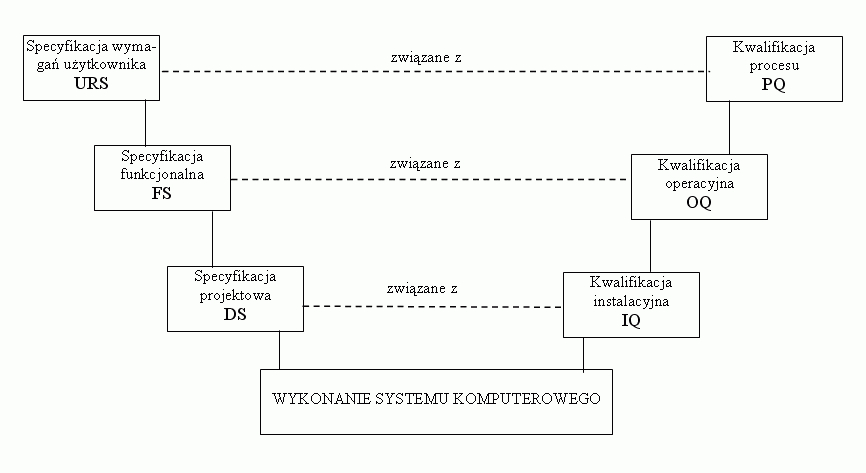
\includegraphics[width=.7\hsize]{images/cykl}
\caption{Cykl życia systemu\label{RYS.3}}
\source{http://www.label.pl}
\end{figure}

Projektowanie systemu skomputeryzowanego można podzielić na kilka etapów:

\begin{enumerate}
  \item \textbf{\textit{Specyfikowanie}} – URS oraz specyfikacja funkcjonalna\footnote{ang. Functional Specification - FS}. W~planie walidacji tego etapu projektowania powinno się uwzględnić audyt dostawcy oraz przegląd specyfikacji.
  \item \textbf{\textit{Projektowanie}} – projekt hardwaru\footnote{ang. Hardware Design System - HDS}, softwaru\footnote{ang. Software Design System - SDS}, projekt mechaniczny i~elektryczny oraz projekt sieci informatycznej. Walidacją objęty jest przegląd poszczególnych projektów – kwalifikacja projektu\footnote{ang. Design Qualification - DQ}.
  \item \textbf{\textit{Wykonanie}} – utworzenie hardwaru, połączeń elektrycznych modułów systemu, oprogramowanie modułów, montaż całego urządzenia, wykonanie sieci informatycznej. Walidacja obejmuje przeglądy wykonania poszczególnych czynności oraz przegląd kodów źródłowych oprogramowania.
\item \textbf{\textit{Testowanie}} – testowanie hardwaru, poszczególnych modułów oprogramowania,  integracji oprogramowania oraz testy funkcjonalne kompletnego urządzenia. Walidacja obejmuje nadzór nad dostawcą poszczególnych elementów systemu.
\item \textbf{\textit{Instalacja}} – instalacja hardwaru, softwaru, urządzeń, sieci informatycznej, testy instalacyjne hardwaru oraz sieci informatycznej. Walidacja tego etapu projektowania systemu skomputeryzowanego dotyczy pełnej kwalifikacji instalacyjnej\footnote{ang. Installation Qualification - IQ}
\item \textbf{\textit{Odbiór}} – testy akceptacji systemu, w~tym kompletności dokumentacji. Na tym etapie realizacji, walidacja dotyczy kwalifikacji operacyjnej\footnote{ang. Operational Qualification - OQ} oraz procesowej\footnote{ang. Performance Qualification - PQ}. Zakończenie jej uwieńczone jest raportem, który powinien określać przykładowo urządzenia produkcyjne, krytyczne parametry procesu i~krytyczne zakresy operacyjne, charakterystykę produktu, sposób pobierania próbek koniecznych do zebrania danych z~badań, ilość przebiegów procesu walidacyjnego i~akceptowalne wyniki badań.
\item \textbf{\textit{Użytkowanie systemu}} – konserwacja i~utrzymanie sprawności systemu, nadzór nad zmianami. W~okresie użytkowania systemu przeprowadzane są okresowe, planowane rewalidacje, a~system jest monitorowany.\cite{LAB-EL2}
\end{enumerate}

\chapter{Elektroniczny indeks}
\indent \indent \indent Elektroniczny indeks jest to elektroniczna platforma, która służy do wystawiania ocen studentom przez prowadzących zajęcia w czasie rzeczywistym, a także do wglądu do tych ocen przez studentów. Dzięki wdrożeniu do użytku wspomnianej platformy, zarówno studenci jak i prowadzący, mogą zaoszczędzić mnóstwo czasu oraz nerwów związanych z próbą zdobycia wpisu, odtworzenia indeksu, gdy zostanie on zgubiony lub uniknięcia długiego stania w kolejce do dziekanatu. Dodatkowo znacznie ułatwiona zostanie biurokracja na lini dziekanat -- wykładowca, a samo zaliczenie semestru studentowi przez osoby do tego uprawnione staję się dużo prostsze i szybsze.

\section{Filtrowanie danych}

\indent \indent \indent Filtrowanie danych w elektronicznym indeksie jest jego ważną częścią. Dzięki temu można uniknąć sytuacji, w której nieautoryzowany użytkownik uzyska dostęp do danych, do których nie powinien miec dostępu. \textit{Meteor} nie ma domyślnie zaimplementowanego pakietu, który pozwoliłby na sprawne zarządzanie dostępnością treści w aplikacji.  Dzięki rosnącej popularności frameworku \textit{Meteor} oraz coraz szerszej grupie deweloperów z każdym dniem pojawiają się nowe pakiety, które ułatwiają i zwiększają funkcjonalność tworzonych aplikacji. Do efektywnego przekazywania danych poszczególnym użytkownikom wykorzystano pakiet \textit{meteor-roles}, który pozwala zarządzać rozsyłanymi danymi oraz jest kompatybilny z wbudowanym pakietem do zarządzania kontami. Instalacja pakietu do zarządzania rolami wymaga dołączenia do projektu pakietu \textit{accounts-password}, co można zrobić nastepującym poleceniem w konsoli:
\newpage
\begin{lstlisting}[language=bash,caption={Instalacja accounts-password}]
	meteor add accounts-password
\end{lstlisting}

Nastepnie możemy dodać właściwy pakiet

\begin{lstlisting}[language=bash,caption={Instalacja pakietu roles}]
	meteor add alanning:roles
\end{lstlisting}


\section{Zarządzanie elektronicznym indeksem przez administratora}

\indent \indent \indent Administrator jest osobą, która nad wszystkim czuwa, dlatego musi mieć dostęp do wszystkich danych i wszystkich funkcjonalności programu, aby móc kontrolować jego poprawność działania. Będąc głównym zarządcą platformy, administrator jako jedyny ma prawo dodawać do systemu nowe dane. Dzięki temu, że najważniejsze dane wyświetlają się administratorowi od razu po zalogowaniu do systemu, jest on w stanie szybko wykonać powierzone mu zadanie.

\begin{figure}[th!]
\centering
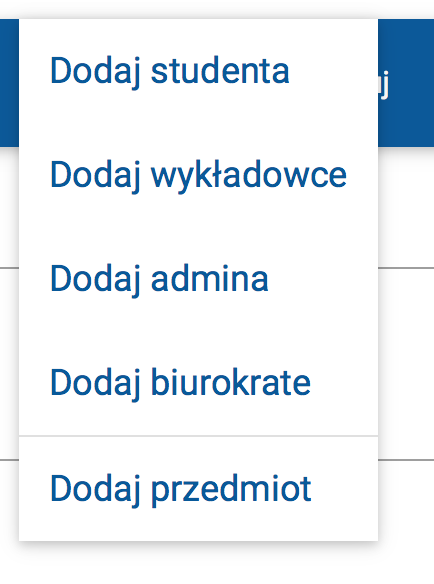
\includegraphics[scale=0.6]{images/menu.png}
\caption{Menu dodawania\label{RYS.4}}
\source{Własne}
\end{figure}


\noindent Jako główny zarządca, administrator ma za zadanie przypisywać studentów do przedmiotów, na które są zobowiązani uczęszczać, a także do przedmiotów, które sami wybiorą w trakcie toku nauczania. Student, który został zapisany na dany przedmiot, nie pojawi się ponownie na liście, dzięki czemu nie ma możliwości zapisania danego użytkownika dwa razy na te same zajęcia.

\begin{figure}[th!]
\centering
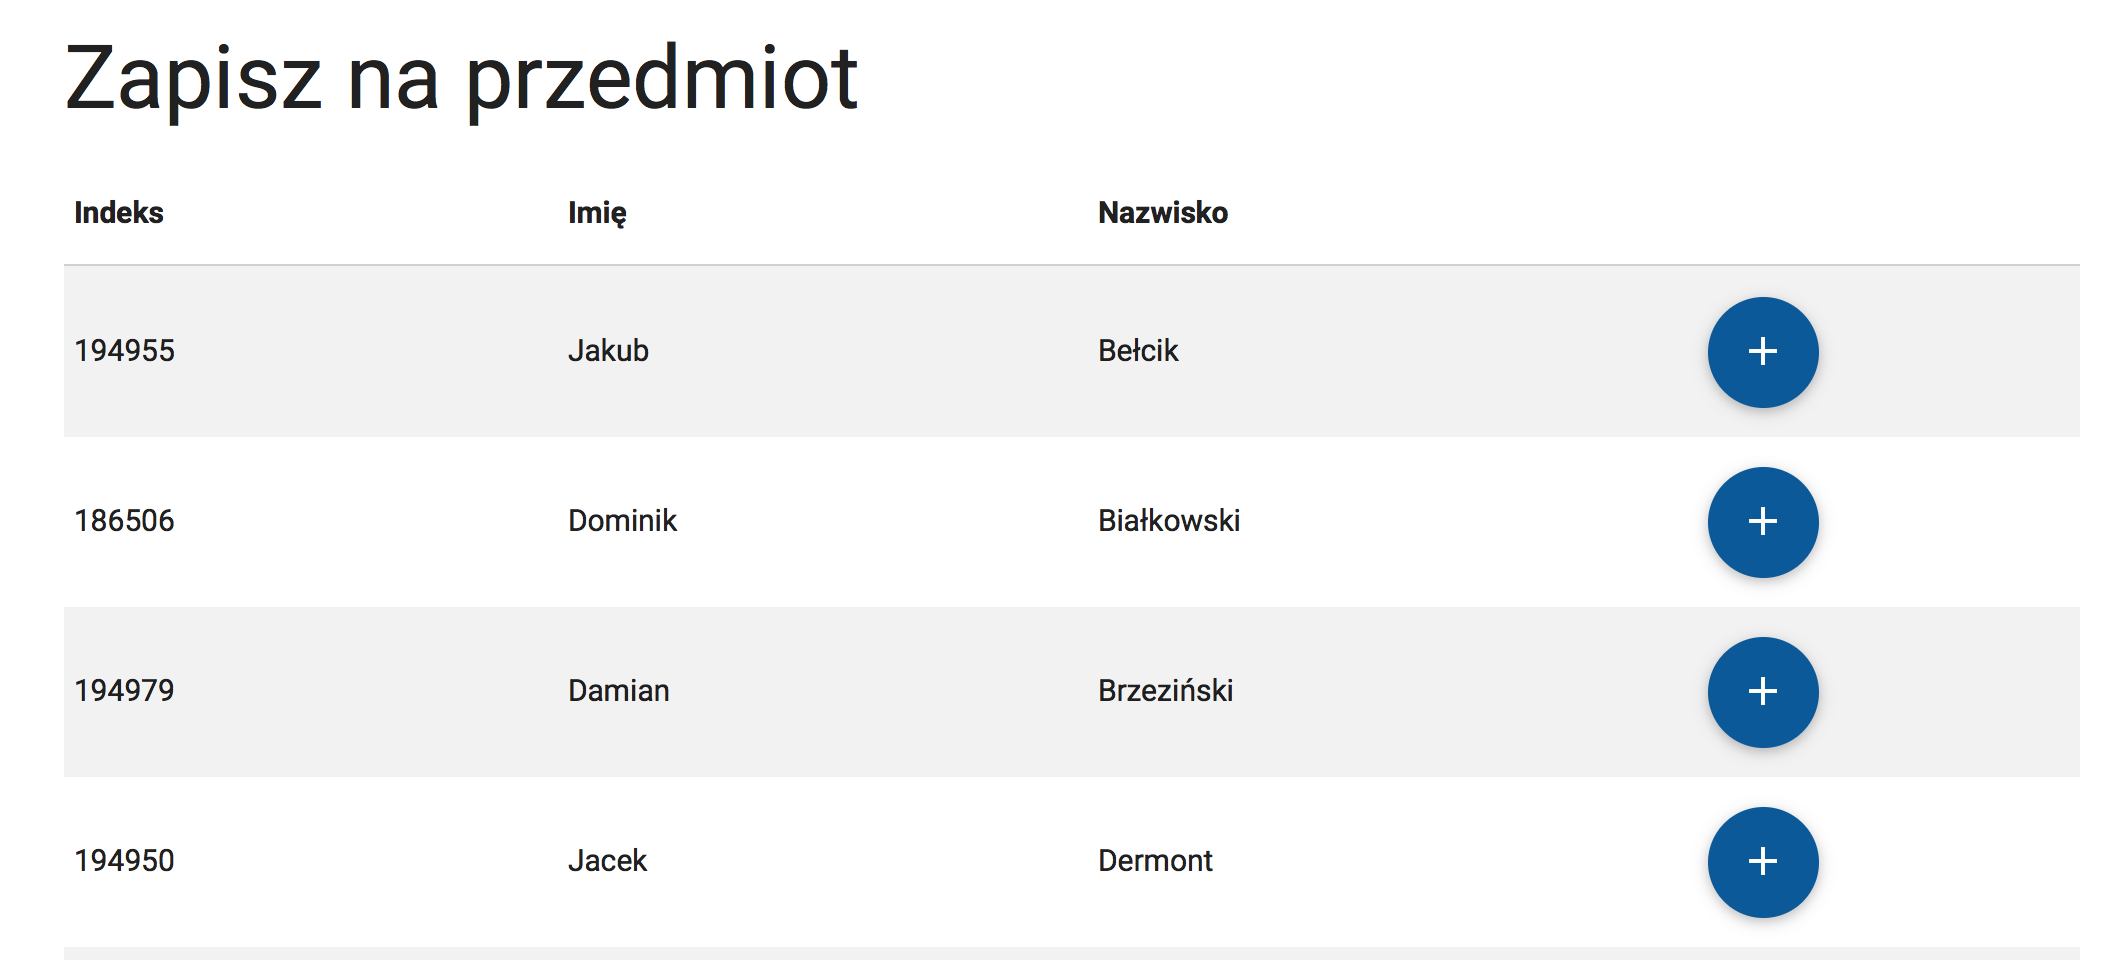
\includegraphics[width=1.1\hsize]{images/addStudent}
\caption{Fragment listy studentów do zapisu na zajęcia\label{RYS.5}}
\source{Własne}
\end{figure}

\noindent Kolejnym zadaniem jest dodawanie przedmiotów, które odbywają się na uczelni. Administrator podaje jego nazwę, wybiera semestr, na którym dane zajęcia się odbywają i z rozwijanej listy wybiera prowadzącego dane wykłady czy ćwiczenia.

\begin{figure}[th!]
\centering
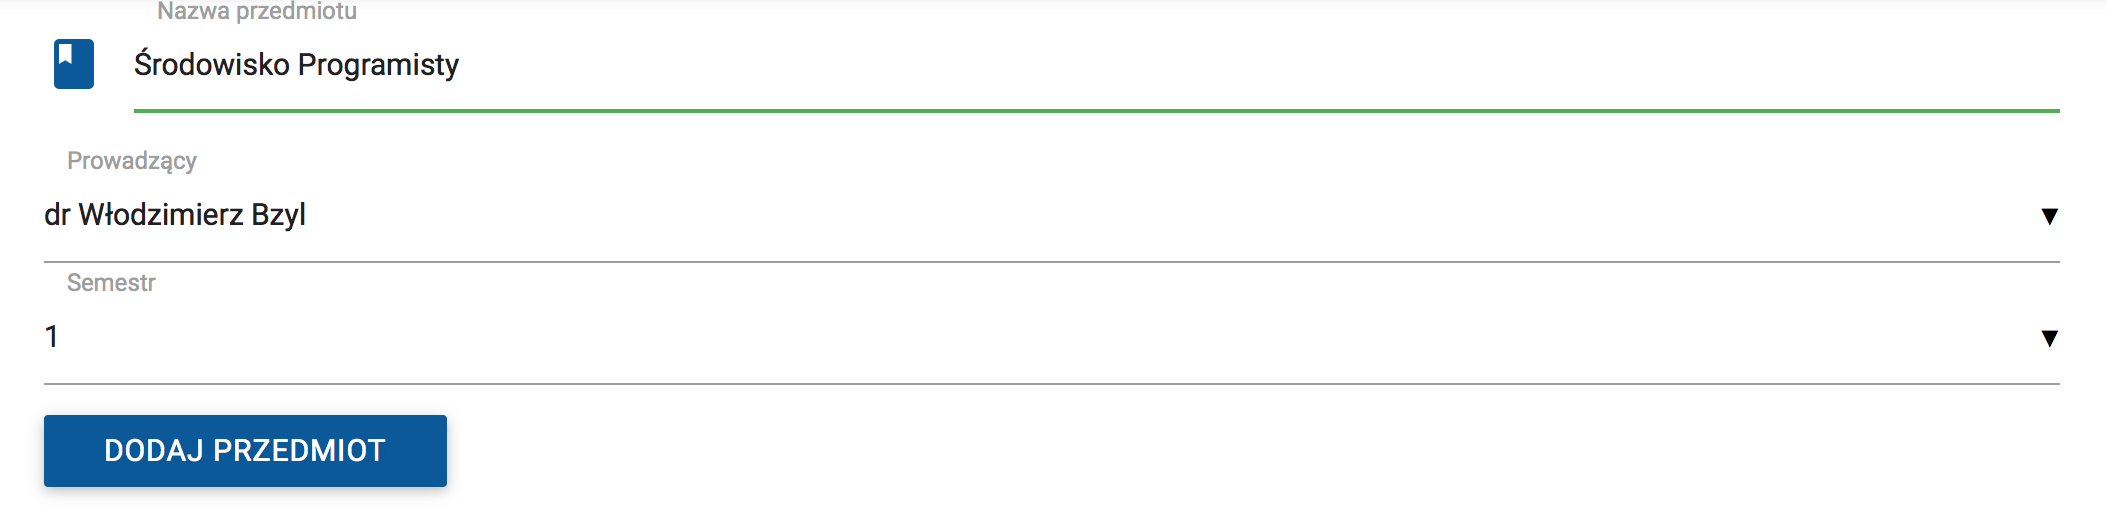
\includegraphics[width=1.1\hsize]{images/addSubject}
\caption{Formularz dodawania przedmiotu\label{RYS.6}}
\source{Własne}
\end{figure}

\newpage

\noindent Następną równie ważną funkcją jest dodawanie studentów, prowadzących zajęcia, adminów oraz pracownków dziekanatu. Z menu dodawania admin wybiera, do jakiej grupy chce dodać użytkownika.

\begin{enumerate}

\item Dodawanie studenta

\begin{figure}[H]
\centering
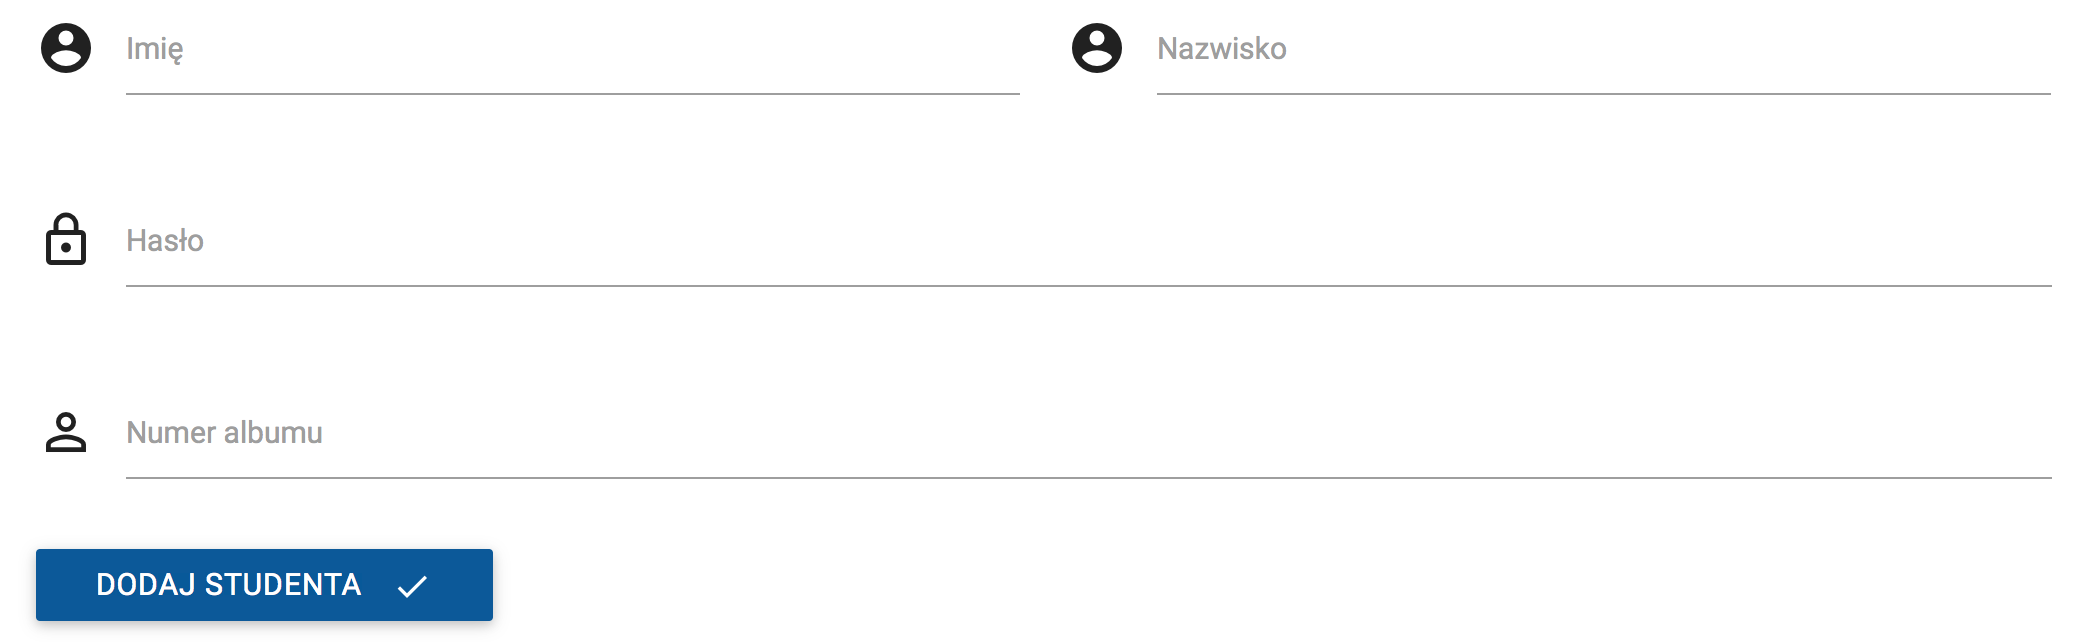
\includegraphics[width=1.1\hsize]{images/addNewStudent}
\caption{Formularz dodawania studenta\label{RYS.7}}
\source{Własne}
\end{figure}

\newpage
\item Dodawanie wykładowcy

\begin{figure}[th!]
\centering
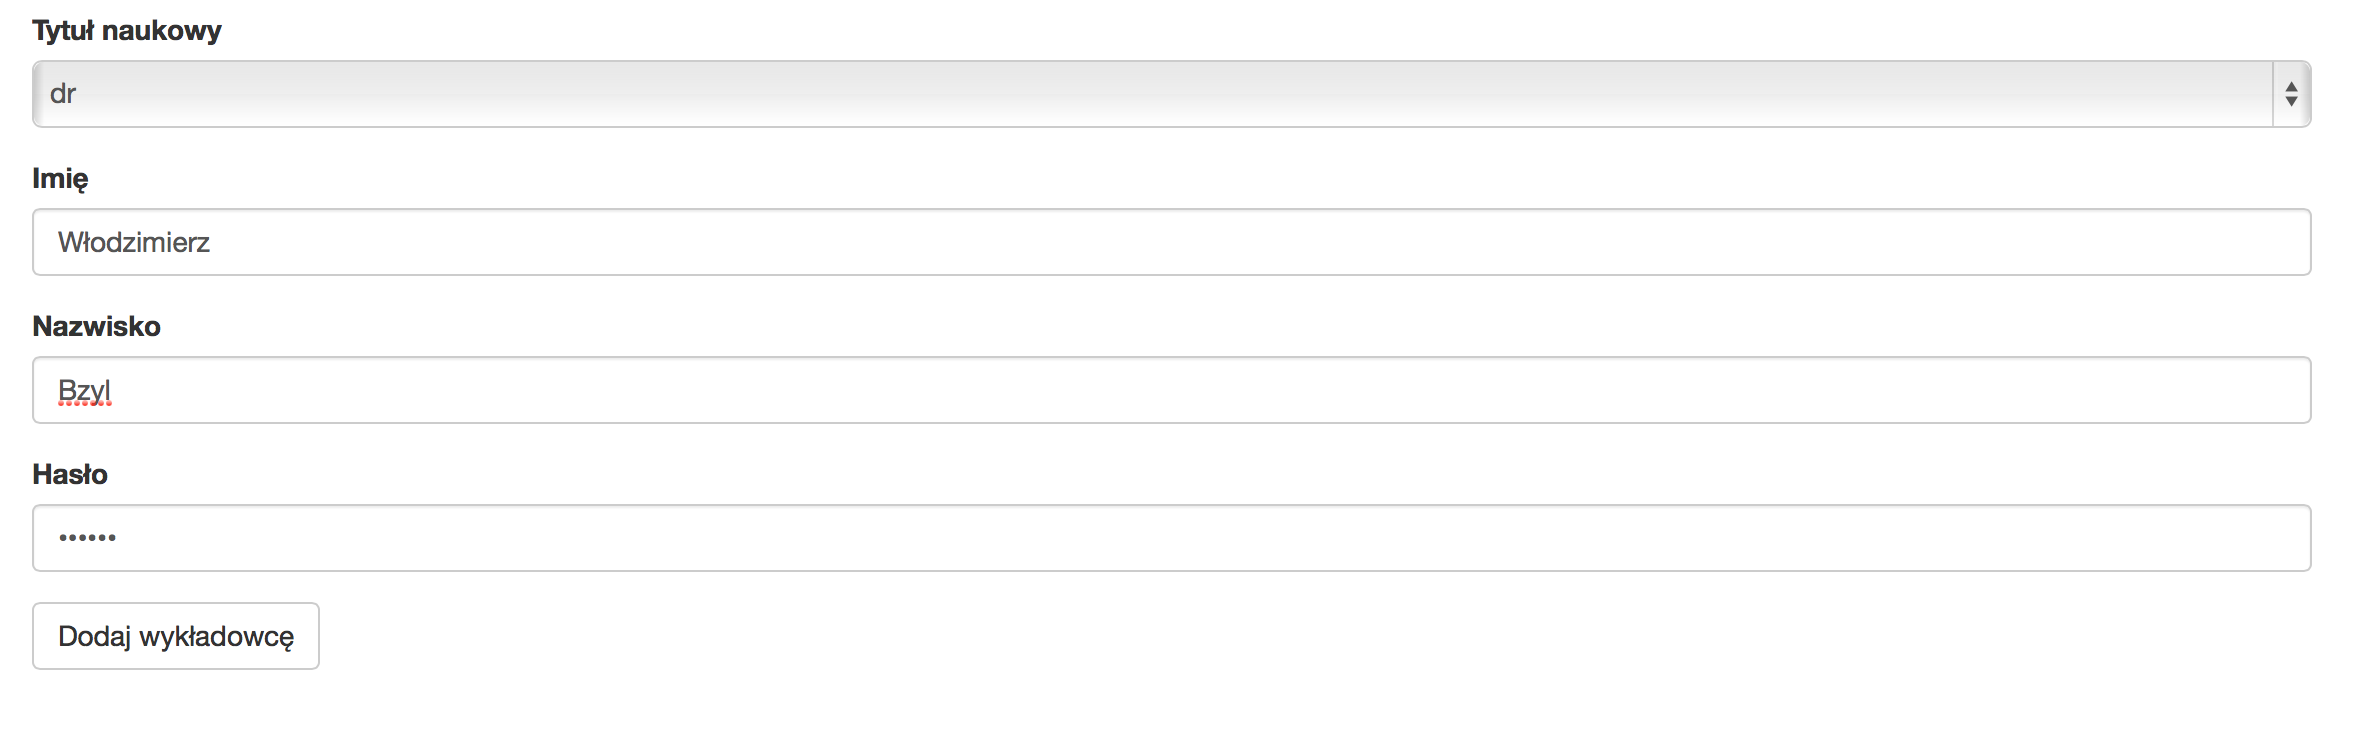
\includegraphics[width=0.9\hsize]{images/addTeacher}
\caption{Formularz dodawania wykładowcy\label{RYS.8}}
\source{Własne}
\end{figure}

\item dodawanie biurokraty

\begin{figure}[th!]
\centering
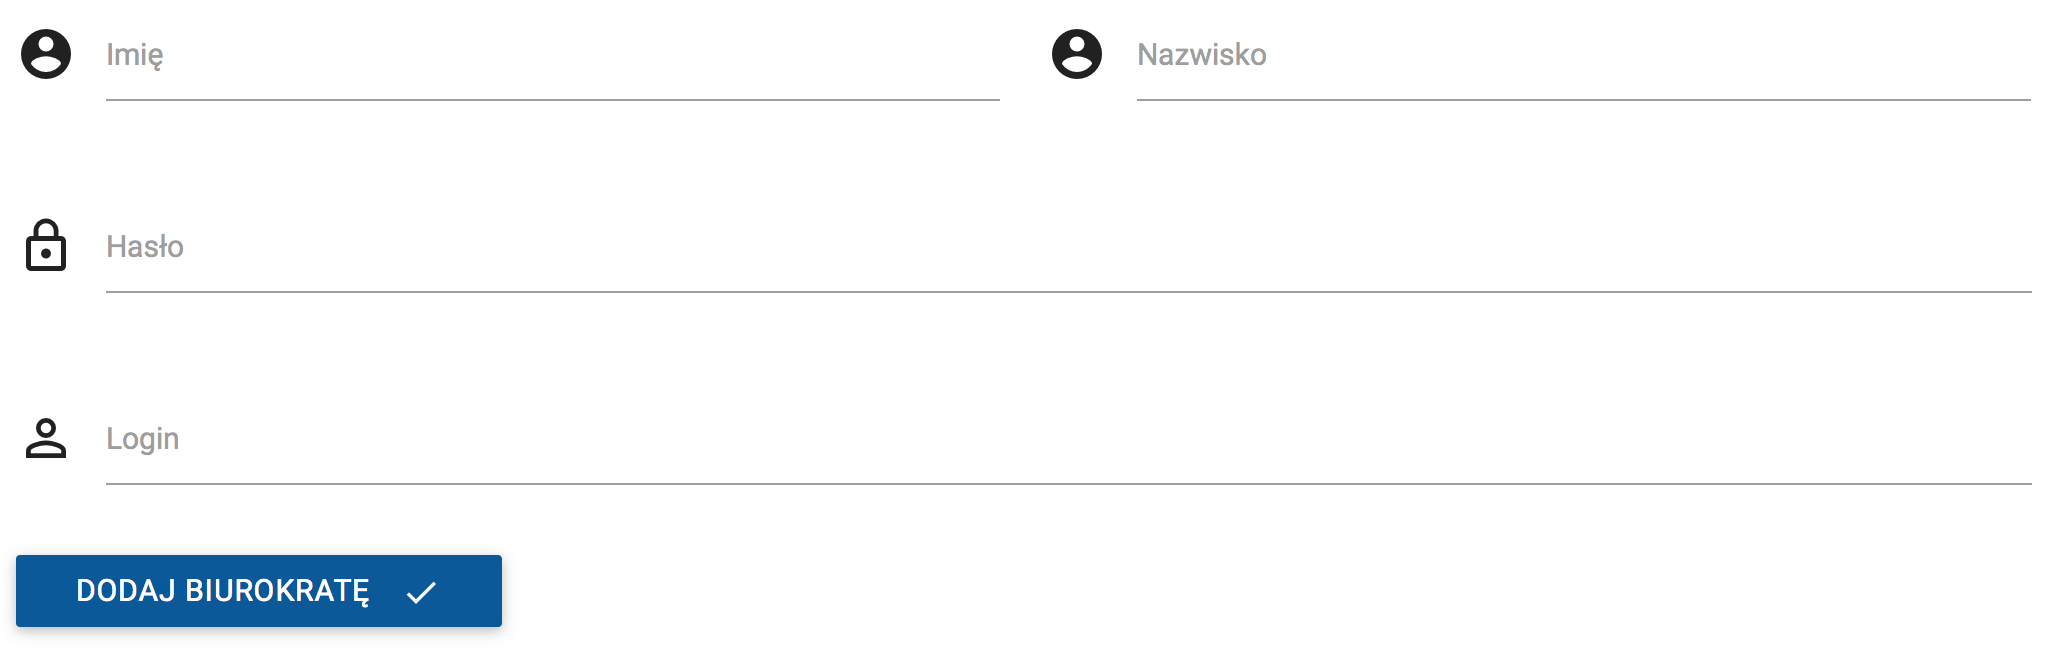
\includegraphics[width=0.7\hsize]{images/addBiurokrata}
\caption{Formularz dodawania pracownika dziekanatu\label{RYS.9}}
\source{Własne}
\end{figure}

\end{enumerate}

\noindent Jako login dla studenta posłuży jego numer albumu, natomiast wykładowca oraz pracownik dziekanatu logować się bedzie do systemu  dzięki loginowi składającemu się z pierwszej litery imienia oraz nazwiska bez używania polskich znaków.

\section{Funkcjonalność dla prowadzącego zajęcia}

\indent \indent \indent Użytkownicy należący do grupy wykładowców muszą mieć możliwość do zarządzania listą studentów, na której widnieją ich nazwiska przypisane do przedmiotów, które prowadzą. Wykładowca ma dostęp wyłącznie do przedmiotów przez siebie prowadzonych. Dzięki temu, podobnie jak w przypadku administratorów, do interesujące wykładowcę dane, można uzyskać w prosty sposób, od razu po zalogowaniu. A prowadzący jest w stanie efektywnie zarządzać swoimi podopiecznymi. Na stronie głównej wykładowca znajdzie listę przedmiotów, które wykłada.

\begin{figure}[th!]
\centering
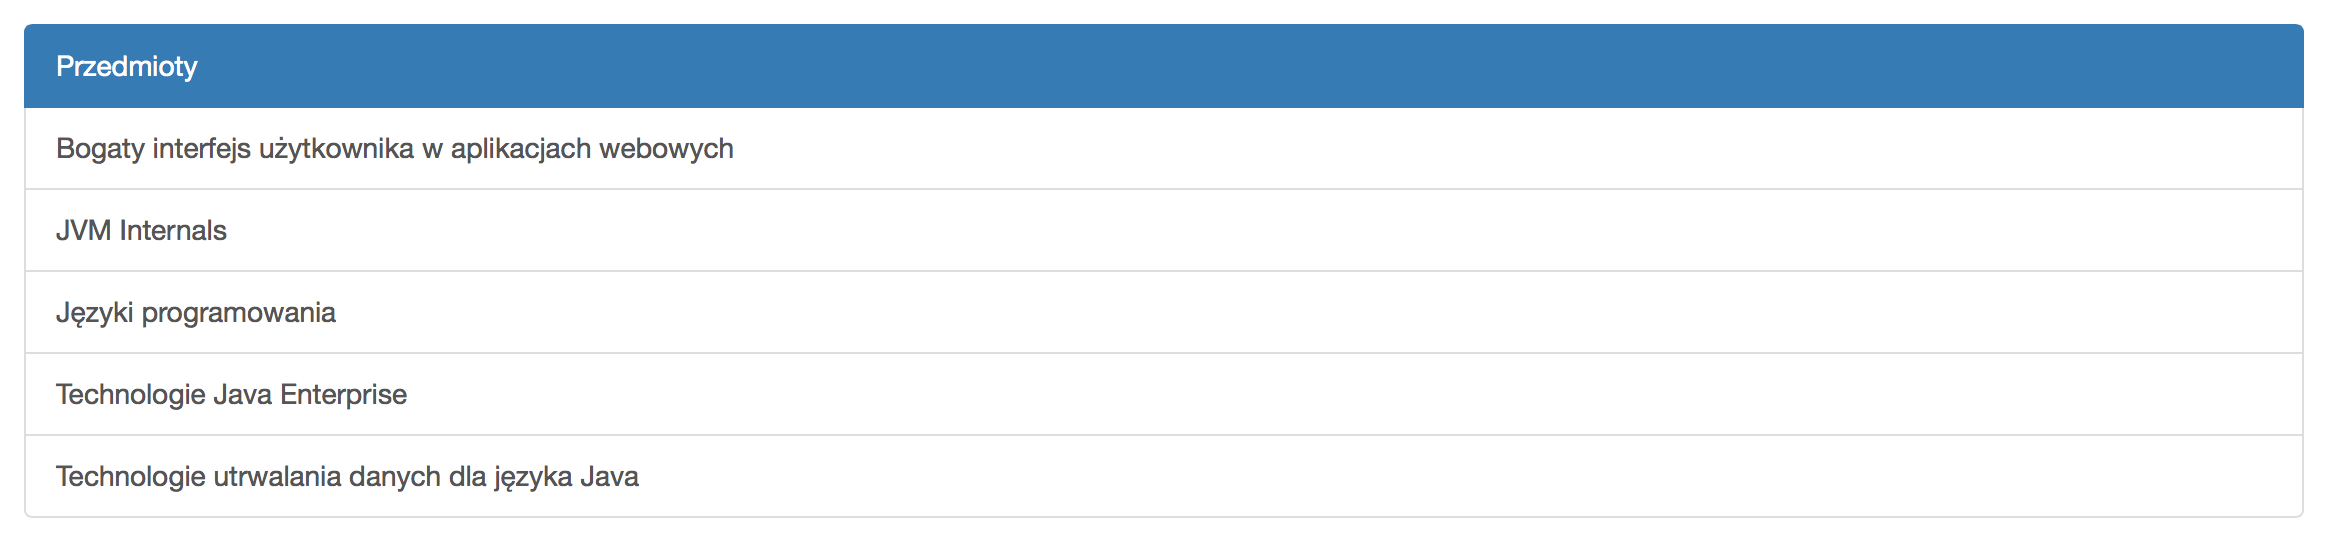
\includegraphics[width=0.7\hsize]{images/subjectList}
\caption{Lista przedmiotów wykładowcy\label{RYS.10}}
\source{Własne}
\end{figure}

\noindent Po wybraniu przez użytkownika interesującego go przedmiotu na ekranie pojawi się lista studentów,  zapisanych na dane zajęcia. Przy każdym uczestniku znajdują się jego imię i nazwisko, numer indeksu oraz rozwijane listy z wyborem oceny za zaliczenie ćwiczeń, a także ocena za egzamin końcowy.

\begin{figure}[th!]
\centering
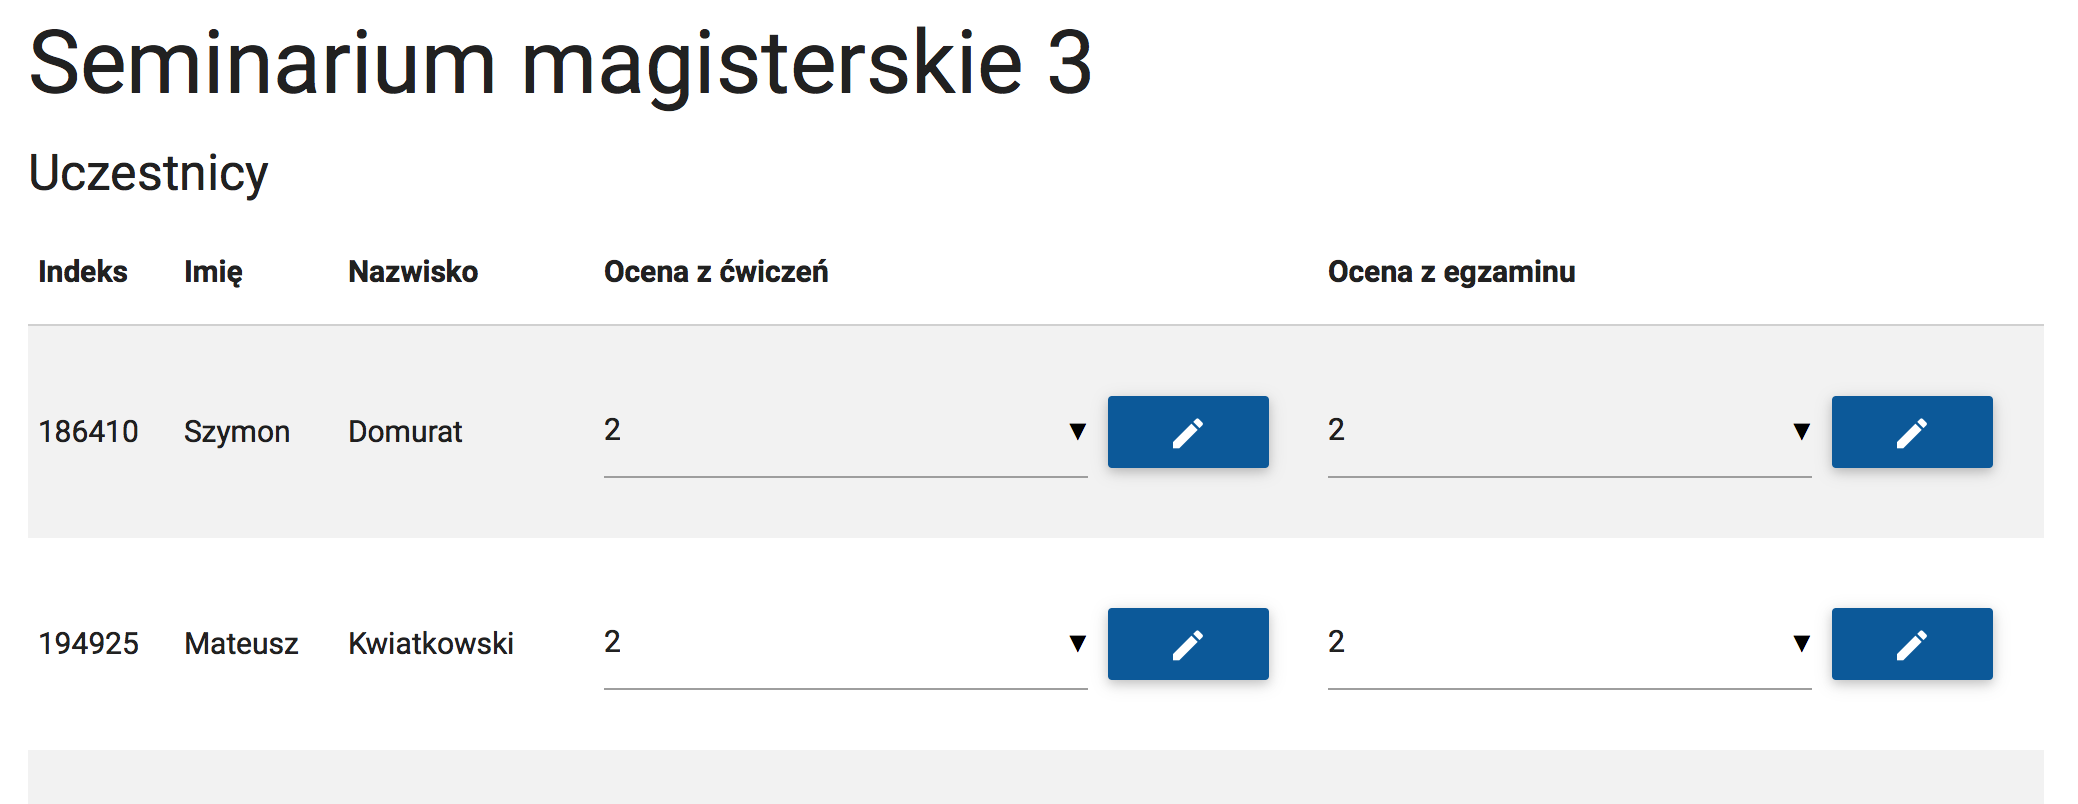
\includegraphics[width=0.7\hsize]{images/studentList}
\caption{Fragment listy studentów zapisanych na przedmiot\label{RYS.11}}
\source{Własne}
\end{figure}

\section{Funkcjonalność dla studenta}
\indent \indent \indent Studenci sa grupą, która ma najmniej do powiedzenia w działaniu aplikacji, ale to studenci najbardziej oczekują szybkiego umieszczenia danych w indeksie. Jedyną funkcjonalnością, z której mogą korzystać studenci, jest przegląd własnych osiągnieć w nauce. Po zalogowaniu do systemu student otrzymuje listę przedmiotów, w których uczestniczy. Po wejściu w interesujacy użytkownika przedmiot, pojawią się informacje o prowadzącym zajęcia, oraz oceny z ćwiczeń i egzaminu.

\begin{figure}[th!]
\centering
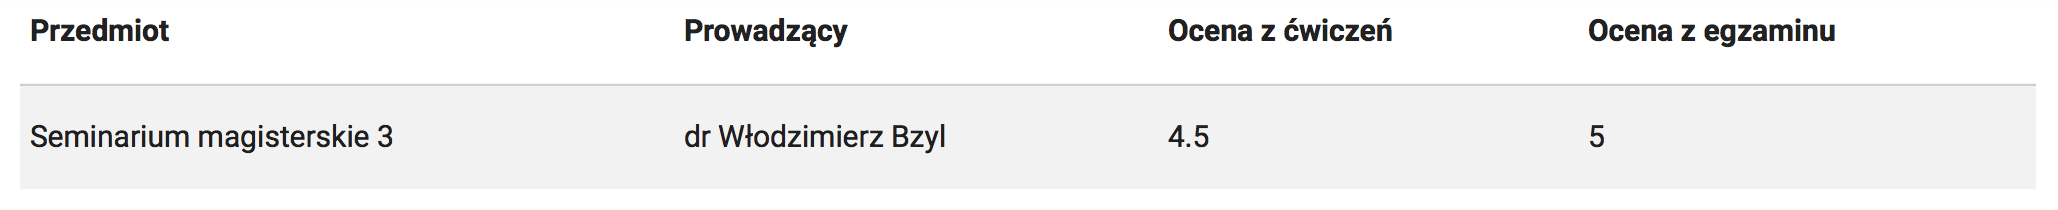
\includegraphics[width=0.7\hsize]{images/studentGrade}
\caption{Oceny studenta z wybranego przedmiotu\label{RYS.12}}
\source{Własne}
\end{figure}

\section{Funkcjonalność dla pracownika dziekanatu}
\indent \indent \indent Kiedy już wykładowca wystawi zaliczenia w elektronicznym indeksie, nadchodzi czas, gdy zarówno wykładowca jak i student, muszą rozliczyć się z tych danych w~dziekanacie. Zadaniem jego pracownika jest utrzymanie porządku oraz spójności danych pomiędzy tymi, które znajdują się w elektronicznej platformie oraz jej papierowym odpowiedniku. Po zalogowaniu do systemu, użytkownikowi pojawi się lista studentów oraz lista wykładowców. Gdy pracownik dziekanatu  wybierze z listy interesującego go studenta, na ekranie pojawi się lista przedmiotów danego ucznia wraz z jego osiągnieciami w nauce, co pozwoli na szybką weryfikację czy dane, które dostarczył student zgadzają się z tymi w aplikacji.

\begin{figure}[th!]
\centering
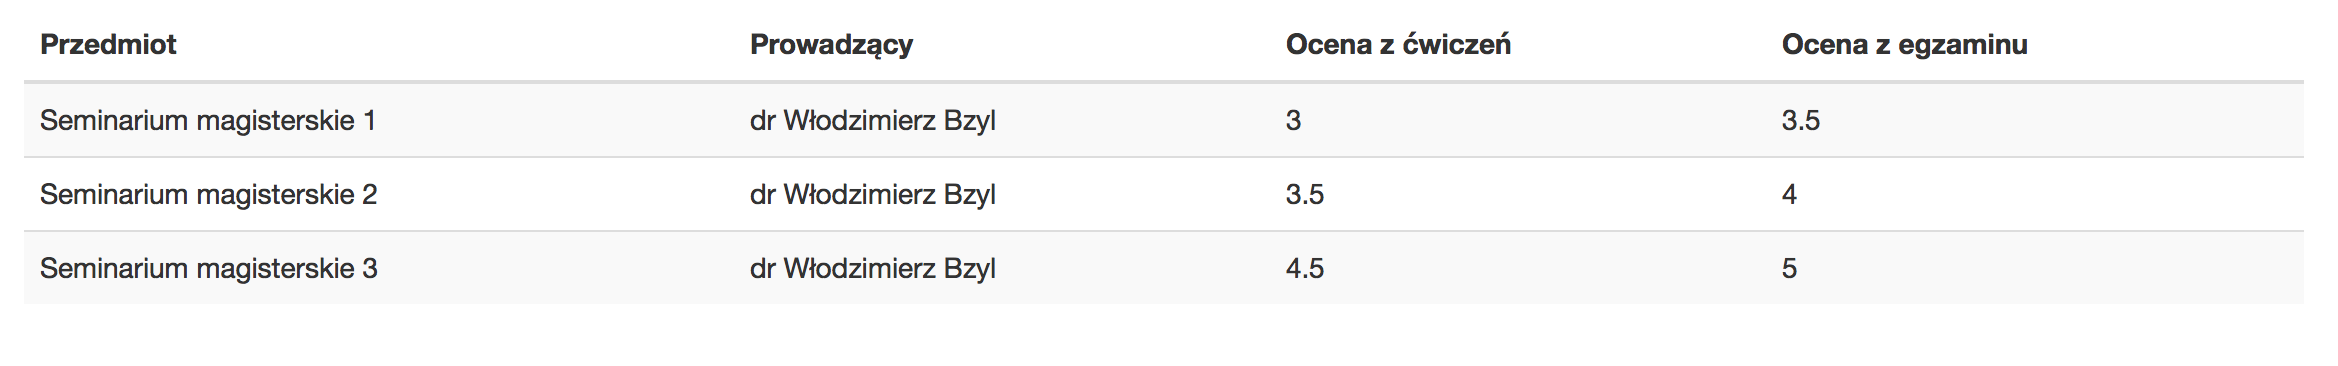
\includegraphics[width=0.7\hsize]{images/studentGrades}
\caption{Oceny studenta\label{RYS.13}}
\source{Własne}
\end{figure}

\noindent Jeśli wybrany zostanie z listy wykładowca, pojawi się na ekranie lista przedmiotów, które dany pracownik prowadzi. Z nowo wyświetlonej listy pracownik dziekanatu może wybrać interesujący go przedmiot, po czym na ekranie pojawią się wszyscy studenci, zapisani na wybrany przedmiot razem ze swoimi osiągnieciami, co pozwoli na szybką weryfikację czy dane dostarczone przez wykładowcę zgadzają się z tymi w elektronicznej platformie.

 \begin{figure}[th!]
\centering
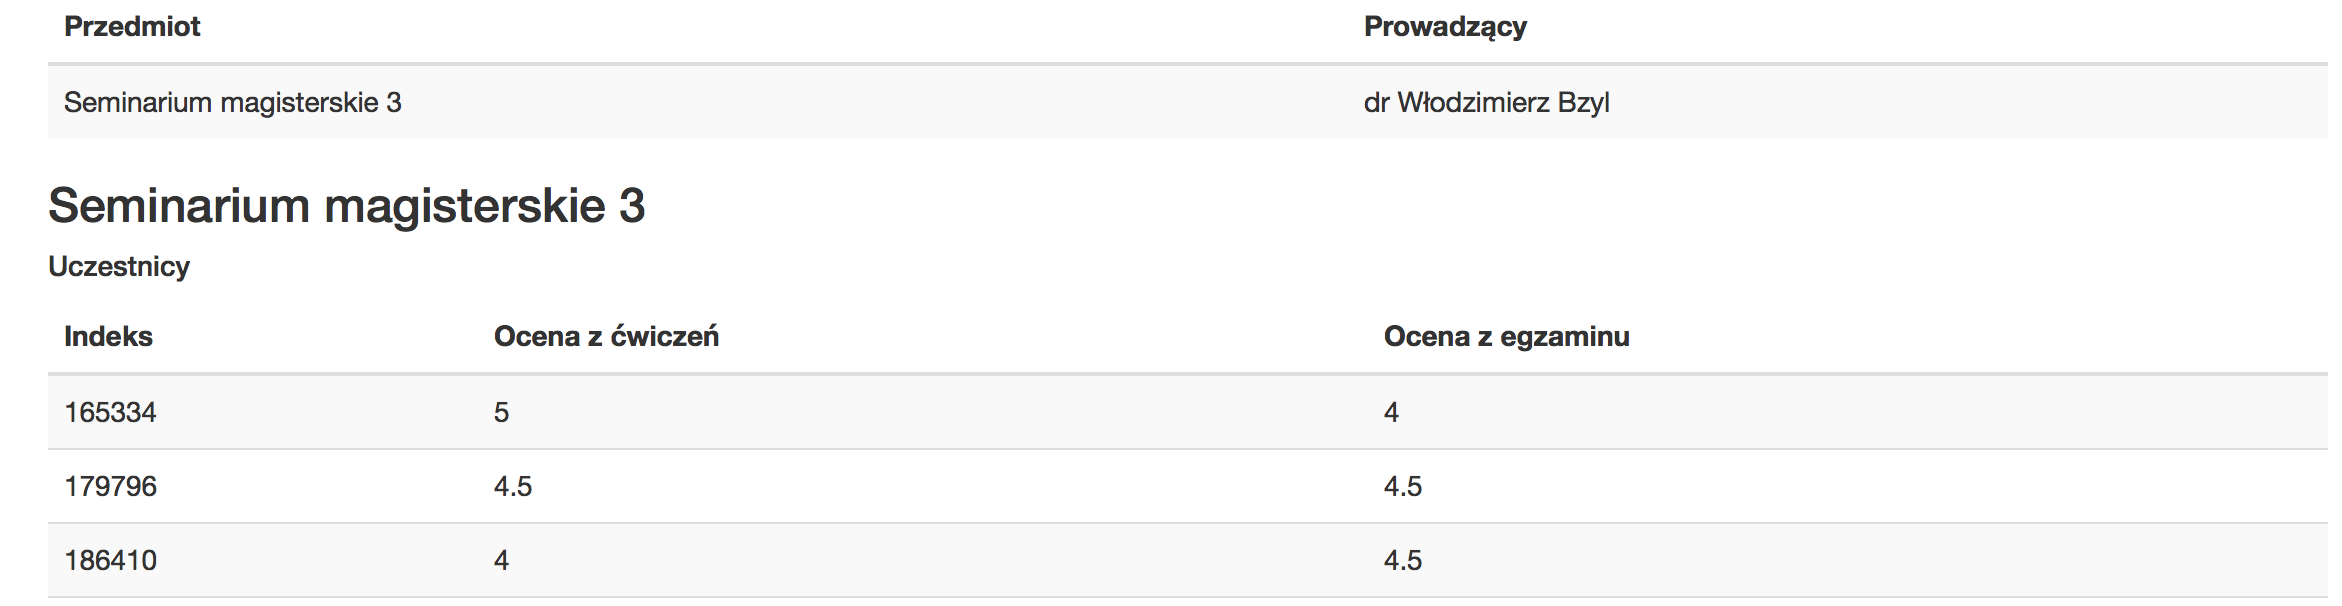
\includegraphics[width=0.61\hsize]{images/deaneryList}
\caption{Fragment listy uczestników zajęć\label{RYS.14}}
\source{Własne}
\end{figure}

\chapter{Aplikacja Elektroniczny indeks w~Meteor}
\section{Opis wybranych technologii użytych w pracy}
\indent \indent \indent Zanim rozpocznie się proces tworzenia aplikacji, programista musi zdecydować, jakich technologii chce użyc do tego celu oraz jakie technologie będą do danego programu najwłaściwsze.
\subsection{Javascript}
\indent \indent \indent Do stworzenia aplikacji - elektroniczny indeks wykorzystano język javascript, którego zaletami są niewielkie rozmiary skryptów, dzięki czemu krótszy jest czas ładowania z serwera, a co za tym idzie mniejsze obciążenie sieci. Dodatkową zaletą jest jego niezależność od systemu, a także nie wymagalność kompilatora.
\subsection{Meteor}
\indent \indent \indent W pracy użyto framework \textit{Meteor} w wersji 1.1.0.2. Jest to framework javascriptowy, który zapewnia aplikacji działanie w czasie rzeczywistym / w skrócie RTA / \footnote{ang. Real-Time Application - RTA}, dzięki czemu użytkownikom korzystającym z aplikacji widoki aktualizują się natychmiast, gdy w bazie danych zachodzą zmiany. Komplementarnie należy podkreślić, że atutetm tej technologii jest fakt, że wszystko, zarówno back-end jak i front-end, piszemy w taki sam sposób, korzystając jedynie z javascriptu. \textit{Meteor} pozwala również zaoszczędzić czas, dostarczając deweloperom gotowe rozwiązania w postaci pakietów. Ich większa część jest wbudowana w framework i wystarczy dodać je do projektu:
\begin{lstlisting}[language=bash,caption={Dodanie standardowego pakietu do projektu}]
	meteor add nazwa_pakietu
\end{lstlisting}
Istnieją również pakiety stworzone przez społeczność, które można przeglądać na \textit{atmosphere.com}. Instalujemy je w bardzo podobny sposób, jak pakiety dostarczone w standardzie:
\begin{lstlisting}[language=bash,caption={Dodanie zewnętrznego pakietu do projektu}]
	meteor add autor:nazwa_pakietu
\end{lstlisting}

\subsection{MongoDB}
\indent \indent \indent \textit{MongoDB} jest najpopularniejszą nierelacyjną bazą danych. Charakteryzuje się dużą skalowalnością, wydajnością oraz brakiem ściśle zdefiniowanej struktury obsługiwanych baz danych. Zamiast tego, dane składowane są jako dokumenty w stylu JSON, co umożliwia aplikacjom bardziej naturalne ich przetwarzanie, przy zachowaniu możliwości tworzenia hierarchii oraz indeksowania. Jest to także obecnie jedyna oficjalnie wspierana baza przez twórców \textit{Meteor}.  W pracy wykorzystana została w wersji 3.0.2.
\subsection{Velocity}
\indent \indent \indent \textit{Velocity} jest oficjalnym narzędziem do testowania aplikacji napisanych w \textit{Meteor} w~wersji 1.0+. Pozwala ono tworzyć testy w popluranych bibliotekach, takich jak: \textit{mocha}, \textit{jasmine}, \textit{cucumber} czy \textit{selenium}. W pracy wykorzystana została biblioteka \textit{jasmine}
\subsection{Distributed Data Protocol}
\indent \indent \indent \textit{Distributed Data Protocol} jest to prosty protokół oparty o format tekstowy \textit{JSON}. Służy on do pobierania danych z~serwera oraz aktualizacji pobranych danych, gdy tylko na serwerze ulegają one zmianie.
\subsection{Roles}
\indent \indent \indent \textit{Meteor-roles} jest to pakiet autoryzujący do frameworka \textit{Meteor}, który pozwala zarządzać, jakie dane zostaną wysłane do konkretnych grup użytkowników.
\subsection{Iron router}
\indent \indent \indent \textit{Iron router} jest to pakiet, którym definiujemy, jak ma wyglądać mapa strony. Działa on zarówno po stronie serwera i klienta. Routing po stronie klienta sprawia, że aplikacja jest naprawdę szybka, gdy już jest załadowana, ponieważ przy każdej zmianie podstrony, nie trzeba jej całej generować.
\subsection{Accounts}
\indent \indent \indent \textit{Meteor account} jest to kompletny pakiet zarządzania kontami użytkowników. Jedną linią kodu można  zapewnić aplikacji możliwość logowania, tworzenia kont, walidacji email, przywracania hasła czy logowania się przez zewnętrzne serwisy jak \textit{facebook} czy \textit{twitter}. Dodatkowo pakiet daje możliwość dostosowania go pod własne potrzeby.
\subsection{Underscore string}
\indent \indent \indent \textit{Underscore.string} jest to pakiet służący do manipulacji stringami. Pierwotnie był rozszerzeniem \textit{Underscore.js}, obecnie jest niezależną biblioteką.

\subsection{Meteor-file-collection}
\indent \indent \indent \textit{Meteor-file-collection} to pakiet, który rozszerza system kolekcji, pozwalając obsługiwać także dane z plików.

\section{Opis tworzenia aplikacji}
\indent \indent \indent Tworzenie aplikacji w frameworku \textit{Meteor} zaczyna się od utworzenia nowego projektu poleceniem w konsoli:
\begin{lstlisting}[language=bash,caption={Tworzenie projektu}]
	meteor create nazwa_projektu
\end{lstlisting}

\noindent Po wykonaniu tej komendy zostanie utworzony folder z projektem, w którym znajdują się trzy pliki.

\begin{figure}[H]
\centering
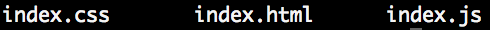
\includegraphics[width=0.8\hsize]{images/newProject}
\caption{Nowy projekt\label{RYS.15}}
\source{Własne}
\end{figure}

Aby skorzystać aplikacji musimy uruchomić lokalny serwer, który pozwoli zobaczyć przetworzony javascript w przeglądarce oraz uruchomić bazę na lokalnym komputerze. W konsoli zmieniamy lokalizację na folder z projektem, a następnie wprowadzamy następującą komendę:

\begin{lstlisting}[language=bash,caption={Uruchomienie aplikacji}]
	meteor run
\end{lstlisting}

\noindent Jeżeli na ekranie pojawi się

\begin{figure}[th!]
\centering
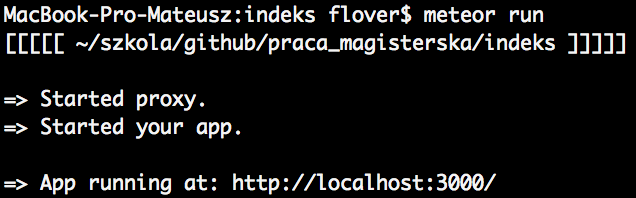
\includegraphics[width=0.8\hsize]{images/succesfullStart}
\caption{Start aplikacji bez błędów\label{RYS.16}}
\source{Własne}
\end{figure}

\noindent oznacza to, że aplikacja uruchomiła się bez błędów i od tego momentu można z niej korzystać pod podanym adresem. Na początku warto podzielić projekt na część serwerową, kliencką oraz dostępną zarówno dla części serwerowej oraz klienckiej.

\begin{figure}[H]
\centering
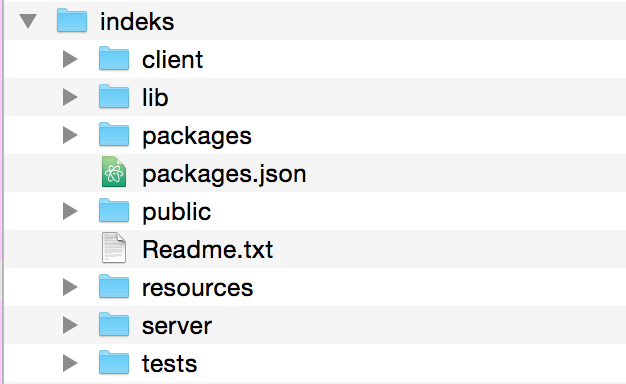
\includegraphics[width=0.75\hsize]{images/splitProject}
\caption{Podział projektu\label{RYS.17}}
\source{Własne}
\end{figure}

Warto również usunąć pakiety \textit{autopublish} oraz \textit{insecure}, dzięki czemu zwiększone zostanie bezpieczeństwo aplikacji. Usnięcie pakietu \textit{insecure} blokuje możliwość użytkownikom do zarządzania bazą danych po stronie klienta, natomiast wyrzucenie \textit{autopublish} spowoduje, że trzeba samemu zadbać o wysyłanie danych z serwera do klienta.\cite{DiscoverMeteor2013}

\begin{lstlisting}[language=bash,caption={Usuwanie pakietów}]
meteor remove autopublish
meteor remove insecure
\end{lstlisting}

W części klienckiej trzymane są widoki aplikacji, funkcje pomocnicze oraz router, a po stronie serwera plik \textit{publish.js}, który definiuje, jakie dane zostną wysłane do użytkowników. Po podzieleniu projektu trzeba utworzyć kolekcje, w których będziemy trzymać informacje o przedmiotach oraz ocenach studentów zdobytych na zajęciach. Do tego celu utworzymy kolekcję subjects, w której będzie trzymana nazwa przedmiotu, tytuł naukowy i nazwisko prowadzącego zajęcia, semestr, na którym przedmiot się odbywa oraz lista zapisanych studentów. Kolekcja grades będzie łączyła informacje z kolekcji z użytkownikami oraz przedmiotami. Znajdą się tu login oraz id użytkownika oraz id przedmiotu, nazwa przedmiotu, jego prowadzący i oceny z ćwiczeń, i egaminu końcowego.

\begin{listing}[H]
\begin{minted}[frame=single]{js}
Subjects = new Mongo.Collection('subjects');
Grades = new Mongo.Collection('grades');
\end{minted}
\caption{Utworzenie kolekcji}
\end{listing}

\noindent Kiedy dysponujemy już kolekcjami, trzeba utworzyć widoki. Zaczynamy od widoku strony głównej, na której w zależności od grupy danego użytkownika, zawierać będzie imiona i nazwiska studentów, poszczególne przedmioty oraz ich wykładowcy.

\begin{listing}[H]
\begin{minted}[frame=single, fontsize=\scriptsize]{html+handlebars}
<template name="subjectList">
  <div class="container">
    <div class="subject-list">
      <div class="list-group">
        {{#if isInRole 'admin, wykładowca, student'}}
        <a class="list-group-item active">
          Przedmioty
        </a>
        {{#if isInRole 'student'}}
        {{#each mySubjects}}
        <a href="/subjects/{{_id}}" class="list-group-item">{{subject}}</a>
        {{/each}}
        {{/if}}
\end{minted}
\caption{Template wyświetlający wszystkie przedmioty, na które uczęszcza student}
\end{listing}

Analogicznie działa wyświetlanie przedmiotów dla wykładowcy czy administratora. W tym momencie, nawet jeśli w bazie będą wprowadzone przedmioty, strona nadal będzie pusta. Do przesyłu danych wykorzystamy \textit{iron-router}.

\begin{listing}[H]
\begin{minted}[frame=single, fontsize=\tiny, breaklines=true]{js}
waitOn: function () {
    return [ Meteor.subscribe('theSubjects') ];
  },
  onBeforeAction: function () {
    if(!Meteor.user()){
      this.layout('appLayout');
      this.render('login');
    }
    else {
      this.next();
    }
  },
action: function () {
    this.layout('appLayout');
    this.render('subjectList', {
      'data': {
        'User': Meteor.user(),
        'mySubjects': Subjects.find(),
        'teacherSubjects': Subjects.find({'leading': Meteor.user().profile.title + " " + Meteor.user().profile.firstName + " " + Meteor.user().profile.lastName}, {sort: {'subject': 1}}),
        'myStudents': Meteor.users.find({'roles': 'student'}, {sort: {'profile.lastName': 1, 'profile.firstName': 1, 'username': 1}}),
        'myLeaders': Meteor.users.find({'roles': 'wykładowca'}, {sort: {'profile.lastName': 1, 'profile.firstName': 1, 'username': 1}}),
        'myGrades': Grades.find()
      }
    });
  }
\end{minted}
\caption{Powyższy fragment renderuje widok z przedmiotami oraz użytkownikami}
\end{listing}

W drugiej linijce kodu widzimy return, który zwraca zasubskrybowane dane z~theSubjects. Żeby te dane można było odebrać, serwer musi je opublikować.

\begin{listing}[H]
\begin{minted}[frame=single, fontsize=\tiny]{js}
Meteor.publish('theSubjects', function () {
  if(this.userId){
    if (Roles.userIsInRole(this.userId, 'admin')) {
      return [Meteor.users.find({}), Subjects.find({})];
    } else if(Roles.userIsInRole(this.userId, 'dziekanat')){
        return [Meteor.users.find({}), Subjects.find({})];
    } else if(Roles.userIsInRole(this.userId, 'student')){
        var user = Meteor.users.findOne({'_id': this.userId})._id;
        return Subjects.find({"students": user});
    } else if(Roles.userIsInRole(this.userId, 'wykładowca')){
        return [Subjects.find({}), Meteor.users.find({})];
      }
    }
    else {
      this.ready();
    }
});
\end{minted}
\caption{udostępnianie danych poszczególnym grupom użytkowników}
\end{listing}

Dzięki pakietowi \textit{meteor-roles} jesteśmy w stanie dokładniej określić, jakie dane chcemy wysyłać poszczególnym grupom użytkowników. Dzięki temu w szybki sposób możemy również zarządzać treściami, które pojawiają się na widokach dzięki blokom pomocniczym.

W aplikacji znajduje się szereg managerów, które przekazują operacje wykonywane przez użytkownika do metod, które zostaną wykonane na serwerze. Funkcja \textit{assignSubject}, która zostaje wywołana w momencie, gdy użytkownik chce przypisać studenta do przedmiotu, pobiera id przedmiotu, jego nazwę, nazwę użytkownika, id użytkownika oraz prowadzącego zajęcia i przekazuje je do metody \textit{addStudentToSubject}, która umieszcza te informacje w kolekcji \textit{grades}, jednocześnie przypisując id studenta do listy osób zapisanych na przedmiot w kolekcji \textit{subjects}. Przypisuje także id przedmiotu do listy przedmiotów, na które student uczęszcza, w~kolekcji użytkowników. Funkcje \textit{updateExerciseGrade} i \textit{updateExamGrade} działają w taki sam sposób. Gdy wykładowca zatwierdza zmianę oceny, pobierają one z pola ocenę, jaką zatwierdził prowadzący, a następnie przekazują id studenta, id przedmiotu oraz ocenę do metod o tych samych nazwach. Dzięki temu, że wysłane zostały także id przedmiotu i studenta, możliwa jest aktualizacja oceny konkretnego studenta dla konkretnego przedmiotu. Gdy administrator wysyła formularz \textit{form}, aby dodać nowy przedmiot, z pól formularza zostają pobrane informacje o nazwie przedmiotu, prowadzącym przedmiot oraz informacja, na którym semestrze zajęcia się odbywają, a następnie są one przesłane do metody \textit{addSubject}, która umieszcza przedmiot w kolekcji \textit{subjects}. W trakcie tworzenia nowego użytkownika, zostaje mu przypisana jedna z czterech dostępnych ról. Jeśli tworzenie użytkownika zakończy się powodzeniem, zostaje wywołana metoda \textit{assignRole}, która otrzymuje stworzonego użytkownika oraz rolę, do której będzie przypisany i ustawia danemu użytkownikowi wybraną rolę.

\cite{Introduction}
\cite{MeteorDocs}
\cite{MongoDocs}
\cite{ScalingMongoDB2011}
\cite{ScalingWithMongoDB}
\section{Opis testowania aplikacji}
\indent \indent \indent Od wersji \textit{Meteor} 1.0, zostało oficjalne udostępnione narzędzie do testowania aplikacji o nazwie \textit{Velocity}. Instaluje się ono razem z jednym z czterech dostępnych frameworków do testowania. W tej pracy użyty został framework \textit{Jasmine}. Aby dodać go do projektu wystarczy w konsoli wpisać

\begin{lstlisting}[language=bash,caption={Instalacja Velocity, Jasmine i html reporter}]
meteor add sanjo:jasmine
meteor add velocity:html-reporter
\end{lstlisting}

\noindent \textit{Html-reporter} jest to reaktywny plugin, który prezentuje wyniki testów.

\begin{figure}[H]
\centering
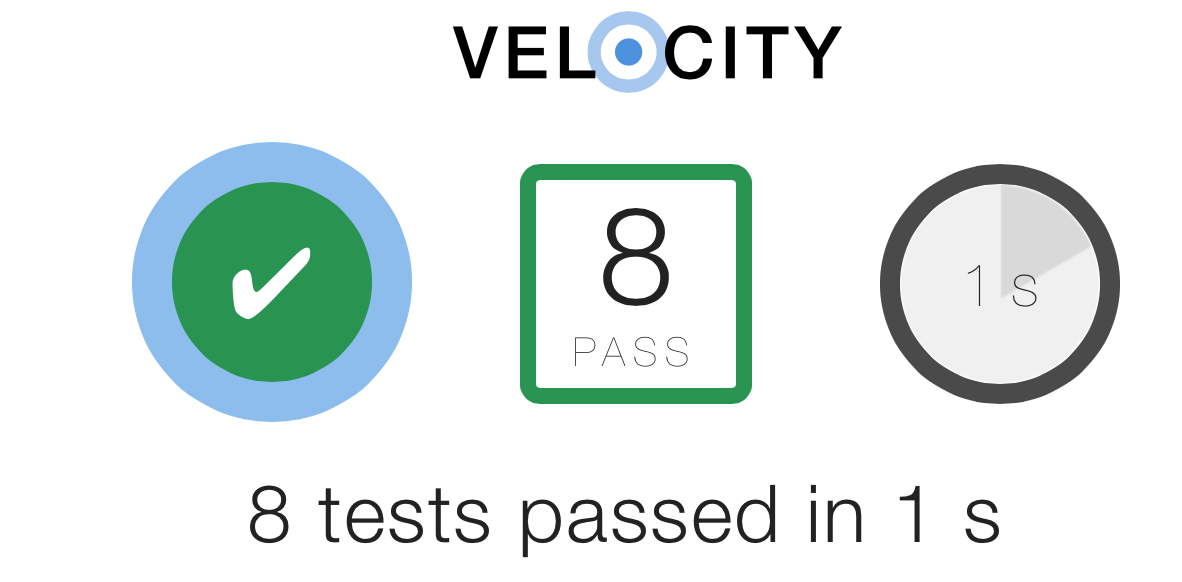
\includegraphics[width=0.7\hsize]{images/htmlReporter}
\caption{Html-reporter\label{RYS.18}}
\source{Własne}
\end{figure}

\begin{listing}[H]
\begin{minted}[frame=single, fontsize=\tiny]{js}
describe('Set user a role', function () {
  it('Should assign user to role', function () {
    if (Meteor.users.find().count() === 0) {
      Accounts.createUser({
        username: 'username1',
        email: 'username1@test.pl',
        password: 'abcdef',
        profile:{
          name: 'student',
          firstName: 'firstName1',
          lastName: 'lastName1',
          subjects:[]
        }
      });
      Accounts.createUser({
        username: 'username2',
        email: 'username2@test.pl',
        password: 'abcdef',
        profile:{
          name: 'student',
          firstName: 'firstName2',
          lastName: 'lastName2',
          subjects:[]
        }
      });
    }

    user = Meteor.users.find({'username': 'username1'}).fetch();

    Meteor.call('assignRole', user[0], 'student');
    expect(Meteor.users.findOne({'username': 'username1'}).roles[0]).toBe('student');

    Meteor.users.remove({'username': 'username1'});
    Meteor.users.remove({'username': 'username2'});
  });

});
\end{minted}
\caption{Test przypisywania roli użytkownikowi}
\end{listing}

\textit{describe} mówi nam, jaka funkcjonalność będzie testowana, \textit{it} opisuje, co dana funkcjonalność powinna robić. Następnie do replikowanej bazy na potrzeby testu dodajemy użytkowników. Gdy użytkowników w bazie, wskazujemy konkretnego użytkownika i pobieramy wszystkie informacje o nim. Wywołujemy metodę, która przypisuje użytkownikowi rolę, a następnie sprawdzamy czy naszemu użytkownikowi została przypisana taka, której oczekiwaliśmy. Po wszystkim czyścimy zreplikowaną bazę. \cite{Velocity}
%\section{Opis własnych rozwiązań}

\chapter{Pakiet walidujący operacje elektronicznego indeksu}
\indent \indent \indent Pakiet ma na celu nie dopuścić do sytuacji,w której użytkownik wprowadzi do bazy danych błędne lub niekompletne treści.
\section{Funkcjonalność pakietu}

\indent \indent \indent Użytkownicy, ktorzy mają dostęp do wprowadzania danych do aplikacji, są szczególnie narażeni na umieszczenie nieprawidłowych informacji w systemie. Dzięki pakietowi dane w aplikacji będą spójne, a użytkownik je modyfikujący będzie miał pewność, że nawet przez pomyłkę nie wprowadzi do systemu błędnych informacji.

\indent Aplikacja stworzona na potrzeby pracy posiada tylko standardową, niezbyt rozbudowaną funkcjonalność, przez co procesowi rozszerzonej walidacji musiały zostać poddane takie operacje, jak: wystawianie zgodnie ze skalą ocen, wystawianie ocen z egzaminu, biorąc pod uwagę czy student spełnił wymagania, aby przystąpić do egzaminu, a także poprawne dodawanie przedmiotów. Do walidacji pól skorzystano z gotowego rozwiązania, pakietu \textit{Mesosphere}
\section{Opis tworzenia pakietu}

\indent \indent \indent Aby utworzyć pakiet, który można będzie wykorzystac w \textit{Meteor}, trzeba w aplikacji utworzyć folder \textit{packages}, a nastepnie w jej  głównym folderze należy użyć polecenia w terminalu bardzo podobnego do tego, którym tworzy się nową aplikację.

\newpage

\begin{lstlisting}[language=bash]
meteor create --package emflover:validation
\end{lstlisting}
\captionof{lstlisting}{Tworzenie nowego pakietu \newline \newline \hspace{\linewidth} \textbf{Interpretacja:} Przełącznik \textit{package} sprawia, że utworzony zostanie pakiet. Jako nazwę przed znakiem dwukropka podajemy swój login dewelopera Meteor, a po dwukropku nazwę pakietu. \newline}

\noindent Jak widać różnicą jest dodanie przełącznika. Jako nazwę przed znakiem dwukropka trzeba podać swój login dewelopera Meteor, a po dwukropku nazwę pakietu.  Po wykonaniu tego polecenia w folderze \textit{packages} zostną utworzone pliki.

\begin{figure}[H]
\centering
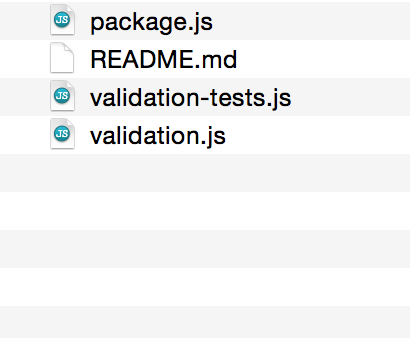
\includegraphics[width=0.7\hsize]{images/newPackage}
\caption{Nowy pakiet\label{RYS.19} \newline \newline \hspace{\linewidth} \textbf{Interpretacja:} \textit{README.md} zawiera opis pakietu; w  \textit{validation.js} mieści się właściwy kod tworzonego pakietu; \textit{validation-tests.js} zawiera testy pakietu; do testowania pakietów służy framework \textit{Tinytest}; \textit{package.js} zawiera opis pakietu oraz jego zależności i gdzie wykonywać mają się poszczególne funkcje.}
\source{Własne}
\end{figure}


\noindent Samo utworzenie nie wystarczy, żeby z niego korzystać. Trzeba go podpiąć do projektu. Podobnie, jak robi się to z~każdym innym pakietem, nawet jeśli nie jest on udostępniony na \textit{atmospherejs.com}.

\cite{Packages}
\cite{MeteorDocs}
\cite{DiscoverMeteor2013}

\section{Implementacja pakietu w~aplikacji}

\indent \indent \indent Tworzenie pakietu wygląda identycznie, jak tworzenie każdej innej funkcji w \textit{javascript}.

\begin{listing}[H]
\begin{minted}[frame=single, breaklines=true,fontsize=\scriptsize]{js}
checkBeforeAction = function(studentId, exercise, exam){
  if(exercise > 2 && exercise <=5){
    Meteor.call('updateExamGrade', studentId, Router.current().params.subjectId, exam);
  } else {
    bootbox.alert("Twoja ocena z ćwiczeń to: " + exercise + ". Nie możesz uczestniczyć w egzaminie.");
  }
}
\end{minted}
\caption{Funkcja spradzająca czy student może otrzymać pozytywną ocenę z egzaminu \newline \newline \hspace{\linewidth} \textbf{Interpretacja:} funkcja przyjmuje trzy argumenty: id studenta, jego ocenę z ćwiczeń oraz ocenę z egzaminu. Jeżeli ocena z ćwiczeń jest negatywna system nie pozwoli na wystawienie pozytywnej oceny studentowi, o czym poinformuje wyskakujące okno z informacją o błędzie. \newline}
\end{listing}

Podajemy nazwę funkcji, przyjmowane argumenty, a następnie podajemy jej ciało. Aby móc skorzystać z nowo stworzonej funkcji, musimy wyeksportować ją z naszego pakietu.

\begin{listing}[H]
\begin{minted}[frame=single, breaklines=true,fontsize=\small]{js}
Package.onUse(function(api) {
  api.versionsFrom('1.1.0.2');
  api.add_files("validation-client.js", "client");
  api.export('checkBeforeAction', 'client');
  api.export('checkIfChooseTeacher', 'client');
});
\end{minted}
\caption{Eksport funkcji i użycie plików, w których znajdują się eksportowane funkcje \newline \newline \hspace{\linewidth} \textbf{Interpretacja:} \textit{versionsFrom} mówi, od jakiej wersji \textit{Meteor} można używać danego pakietu; \textit{add\_files} dodaje pliki, w których znajduje się kod pakietu oraz mówi czy ma być przesłany do serwera, czy klienta; \textit{export} - jak sama nazwa wskazuje, eksportuje funkcje z dodanego wcześniej pliku i określa, czy mają zostać wykonane po stronie serwera czy klienta.  \newline}
\end{listing}

Aby użyć pakietu w aplikacji musimy, wywołać ją po stronie klienta.

\begin{listing}[H]
\begin{minted}[frame=single, breaklines=true,fontsize=\scriptsize]{js}
'click .updateExamGrade': function (event, template) {
    var examGrade = template.find('#subjectExamGrade_'+this._id).value;
    var exerciseGrade = Grades.findOne({'subjectId': Router.current().params.subjectId, 'studentId': this._id}).exerciseGrade;
    checkBeforeAction(this._id, exerciseGrade, examGrade);
  }
\end{minted}
\caption{Funkcja wystawiająca studentowi oceny \newline \newline \hspace{\linewidth} \textbf{Interpretacja:} Funkcja pobiera wartość pola z oceną z egzaminu oraz pobiera z bazy ocenę studenta z ćwiczeń i przekazuje je do funkcji walidującej. \newline}
\end{listing}

Podczas wystawiania oceny do funkcji przekazane zostają id użytkownika, któremu wystawiana jest ocena, ocena jaką wykła%dowca chce wystawić studentowi z egzaminu oraz wcześniejsza ocena studenta z ćwiczeń.

\section{Przetestowanie pakietu}

Do testowania pakietów \textit{Meteor} służy framework \textit{TinyTest}. Jest to oficjalne i jedyne narzędzie służące do przeprowadzania testów pakietów. Wadą tego frameworka jest fakt, że nie został on w żaden sposób opisany, przez co korzystanie z niego dla osoby niedoświadczonej może być nie do końca zrozumiałe.
\newline \newline
Aby przetestować pakiety, należy w głównym folderze aplikacji wpisać w konsoli polecenie:

\begin{lstlisting}[language=bash]
meteor test-packages ./packages/validation/
\end{lstlisting}
\captionof{lstlisting}{Testowanie pakietu \newline \newline \hspace{\linewidth} \textbf{Interpretacja:} \textit{test-packages} mówi o tym, że uruchamiamy testy pakietu; \textit{./packages/validation/} jest to ścieżka do testowaneo pakietu\newline}

Po wykonaniu polecenia, jeżeli stworzone testy nie zawierają błędów, uruchomi się serwer, na którym zostaną one przeprowadzone, a wyniki zostaną przedstawione na czytelnym interfejsie użytkownika. Jeśli test zostanie wykonany prawidłowo, na ekranie wyświetli się:

\begin{figure}[H]
\centering
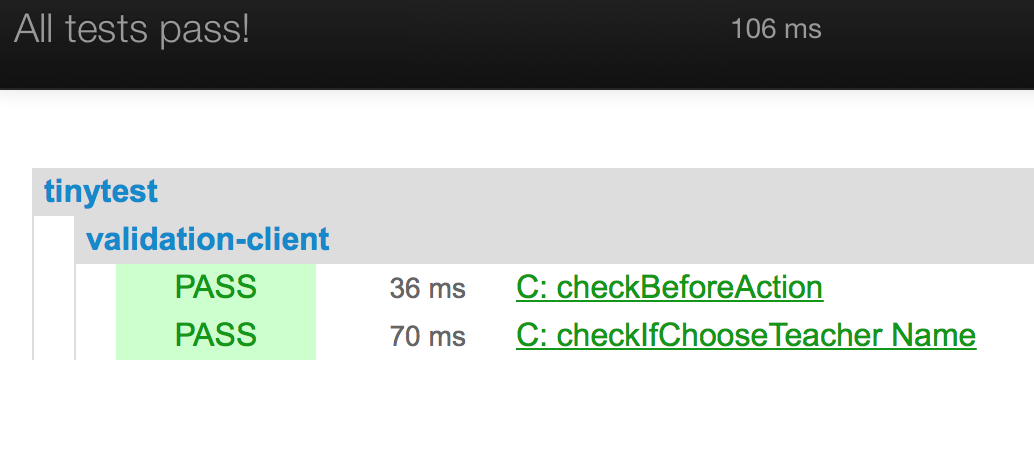
\includegraphics[width=0.7\hsize]{images/tinytestSucced}
\caption{Wynik testów bez błędów\label{RYS.20} \newline \newline \hspace{\linewidth} \textbf{Interpretacja:} Testy po stronie klienta zakończyły się sukcesem.}
\source{Własne}
\end{figure}

Jeżeli w teście będą błędy i zostanie otrzymany wynik odbiegający od oczekiwań, na ekranie pojawi się:
\begin{figure}[H]
\centering
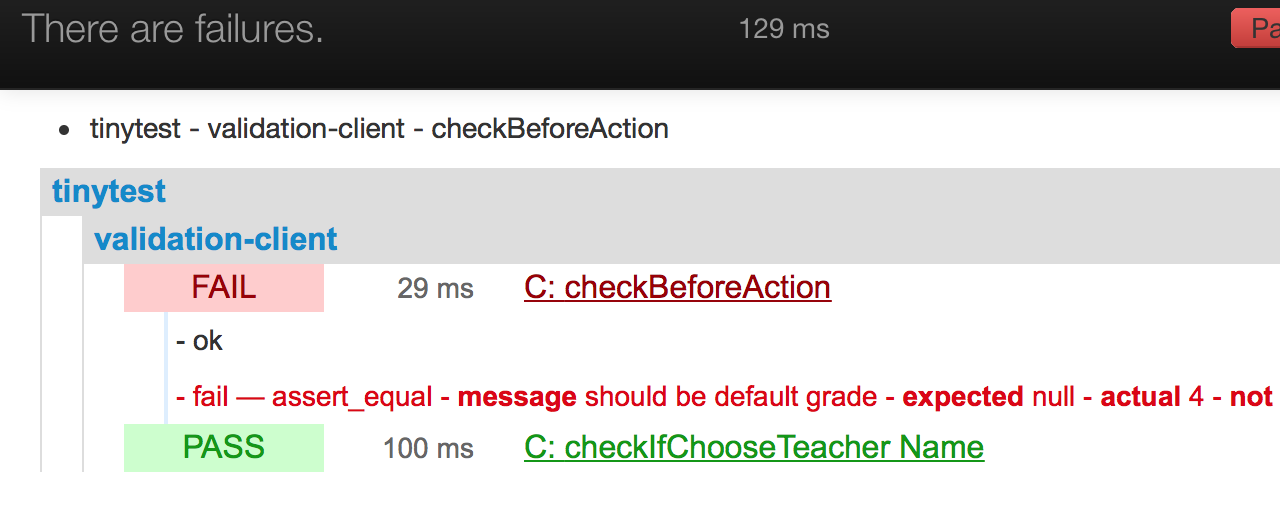
\includegraphics[width=0.7\hsize]{images/tinytestFailure}
\caption{Wynik testów zakończone niepowodzeniem\label{RYS.21} \newline \newline \hspace{\linewidth} \textbf{Interpretacja:} Test \textit{checkBeforeAction} zakończył się niepowodzeniem. Oczekiwano wartości null, natomiast funkcja zwróciła 4.}
\source{Własne}
\end{figure}

Aby wykonać test, musimy w pliku \textit{package.js} dodać:

\begin{listing}[H]
\begin{minted}[frame=single, breaklines=true,fontsize=\scriptsize]{js}
Package.onTest(function(api) {
  api.use('tinytest');
  api.use(['mizzao:bootboxjs']);
  api.use('emflover:validation');
  api.addFiles('validation-tests.js');
});
\end{minted}
\caption{Zależności potrzebne do testowania aplikacji \newline \newline \hspace{\linewidth} \textbf{Interpretacja:} \textit{api.use} pobiera pakiety, które będą potrzebne do poprawnego przeprowadzenia testu; \textit{api.addFiles} dodaje pliki potrzebne do wykonania testu. \newline}
\end{listing}

Pomimo tego, że w projekcie mamy dodane potrzebne pakiety, podczas przeprowadzania testów \textit{tinytest} nie jest w stanie z nich skorzystać, jeśli sami nie wskażemy, że odpowiednie narzędzia są dostępne.

\begin{listing}[H]
\begin{minted}[frame=single, breaklines=true,fontsize=\scriptsize]{js}
Tinytest.add('validation-client - checkBeforeAction', function (test) {
    var exerciseGrade = 2;
    var examGrade = 3;
    var Person = function(id, username){
      this.id = id;
      this.username - username;
    }
    var Subject = function(id, subjectName, leading){
      this.id = id;
      this.subjectName = subjectName;
      this.leading = leading;
    }
    var Grade = function(id, subjectId, studentId, exercise, exam){
      this.id = id;
      this.subjectId = subjectId;
      this.studentId = studentId;
      this.exercise = exercise;
      this.exam = exam;
    }
    var student = new Person('1', 'username1');
    var sub = new Subject('1', 'Subject 1', 'Leading 1');
    var gradez = new Grade('1', '1', '1', exerciseGrade, null);
    checkBeforeAction('1', exerciseGrade, examGrade);
    test.equal(gradez.exercise, 2, 'Should be grade 2');
    test.equal(gradez.exam, null, 'should be default grade');
}
\end{minted}
\caption{Test dodawania oceny z egzaminu studentowi gdy ma on negatywną ocenę z ćwiczeń \newline \newline \hspace{\linewidth} \textbf{Interpretacja:} Pierwszym argumentem \textit{Tinytest.add} jest nazwa naszego testu, a drugim  funkcja, która go wykona. Na potrzeby testu definujmey i tworzymy nowego użytkownika, przedmiot oraz ocenę, a następnie wywołujemy testowaną funkcję, a po jej wykonaniu sprawdzamy czy oceny z ćwiczeń i egzaminu się zgadzają.\cite{TinyTest}  \newline}
\end{listing}



% zakończenie
\summary
\indent \indent \indent Celem pracy magisterskiej było stworzenie aplikacji - elektroniczny indeks oraz pakietu, który walidował operacje wykonywane podczas użytkowania oprogramowania. Cele pracy zostały osiągnięte, dając zadowalające rezultaty.
\newline \newline
Technologie wykorzystane w pracy okazały się dobrym wyborem, ponieważ oferowały szeroki wachlarz narzędzi, które usprawniały pracę nad projektem, pozwalały w niedługim czasie stworzyć aplikację, która posiadała wymaganą podstawową funkcjonalność, dzięki czemu można było ją przetestować i walidować.
\newline \newline
Podczas tworzenia pracy pojawiły się problemy ze strony dostarczonych technologii. Dla sprawnego przeglądu informacji przez użytkowników, autor chciał sortować dane wyświetlane użytkownikowi leksykograficznie, na co pozwala \textit{MongoDB}, ale technologia ta ze względu na wykorzystywaną funkcję \textit{memcmp} nie obsługuje poprawnie formatu UTF-8 w różnych ustawieniach lokalnych. Twórcy bazy danych planują wprowadzić zmiany w systemie, ale przybliżona data nie jest znana, ponieważ wymaga to wielu poważnych modyfikacji programu.
\newline \newline
Niewątpliwą zaletą systemu jest możliwość jego rozdudowy bez konieczności ingerencji w kod, który został napisany wcześniej, czego dowodem jest dodanie funckji pobierania danych z aplikacji oraz ich import z powrotem do systemu z poziomu aplikacji, już po zakończeniu jej tworzenia. Ta dodatkowa funkcjonalność pozwala użytkownikom zarządzać danymi w swoich własnych aplikacjach typu - elektroniczny indeks, utworzonym przez nich na własne potrzeby.

% załączniki (opcjonalnie):
%\appendix


% literatura (obowiązkowo):
\bibliographystyle{unsrt}
\bibliography{mgr}

% spis tabel (jeżeli jest potrzebny):
%\listoftables

% spis rysunków (jeżeli jest potrzebny):
\listoffigures

\oswiadczenie

\end{document}
